% \begin{savequote}[8cm]
% Conoscere nel senso della Scienza vuol dire prevedere.

% To know in its Scientific meaning, means to predict.
%   \qauthor{--- Carlo Rubbia}
% \end{savequote}

\chapter{\label{ch:3-DUNE}The Deep Underground Neutrino Experiment}


\minitoc
\section{Introduction} \label{ch3-Sec:Introduction}
\begin{figure}[!ht]
     \centering
     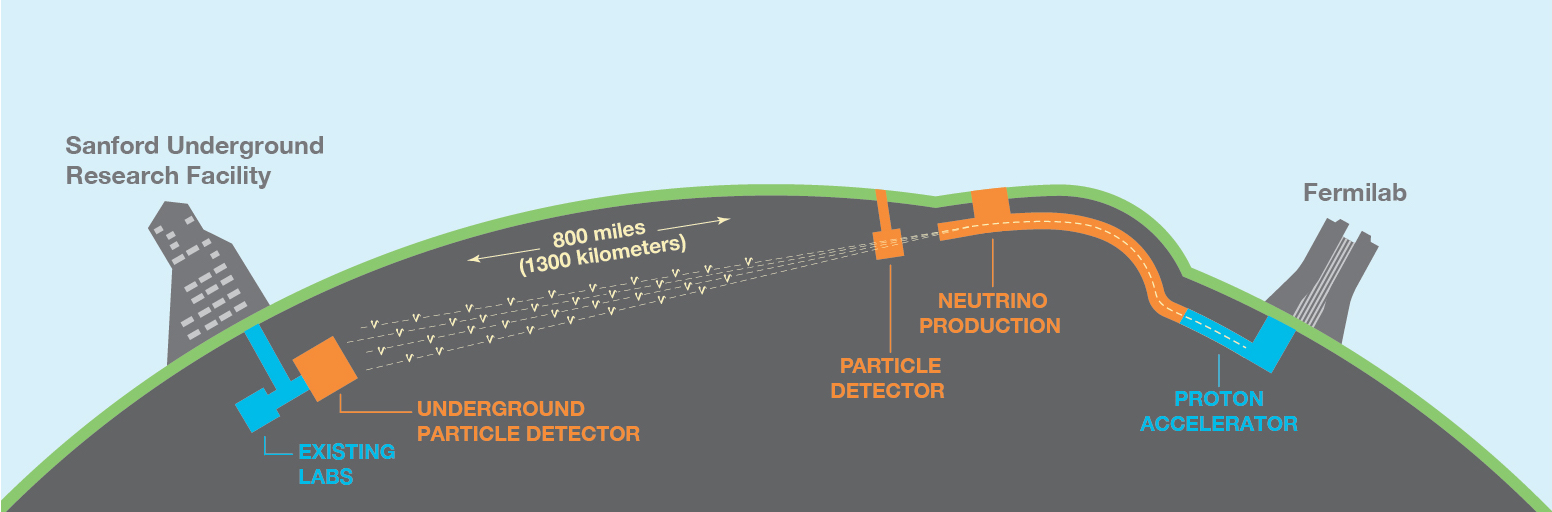
\includegraphics[width=0.99\textwidth]{figures/ch3-DUNE/LBNE_Graphic_061615_2016.jpg}
     \caption[Schematic representation of the DUNE experiment.]{Schematic representation of the DUNE experiment with its main components \cite{DUNE:2020TDR1}.}
        \label{fig:DUNEdiagram}
\end{figure}
The Deep Underground Neutrino Experiment (DUNE) will be a next generation long baseline neutrino oscillation experiment \cite{DUNE:2020TDR1}. Its main goal will be to measure all the parameters governing neutrino and anti-neutrino oscillations in a single experiment, with particular emphasis on the CP violation phase $\delta_\textrm{CP}$ and the neutrino mass ordering. The experiment will consist of three main components: a wide band high intensity neutrino beam situated at Fermilab, which will be capable of producing both a $\nu_\mu$ and a $\Bar{\nu}_\mu$ fluxes; a kt-scale underground liquid Argon based far detector (FD), situated at the Sanford underground research facility (SURF) in South Dakota, at $\sim1300$ Km from the source; a modular near detector (ND) situated at $\sim500$ m from the source. 

In this chapter we start by providing an overview of the DUNE's facilities in Section \ref{Sec:DUNEfacilities}. A dedicated discussion of the muon spectrometer component of the experiment's ND, which is the focus of this thesis, is then provided in Sections \ref{sec:DUNE-ND-GAr} and \ref{Sec:TMS}. An overview of the experiment's scientific program is then offered in Section \ref{Sec:DUNEscientific} with a final discussion dedicated to the physics goals of the near detector in Section \ref{Sec:NDScientific}.  



\section{DUNE's facilities and design}
\label{Sec:DUNEfacilities}

In this section we give a brief overview of the components constituting the DUNE experiment, including the neutrino beamline, the Near Detector and the Far Detector. Due to budgetary restrictions DUNE will pursue a staged approach in its construction and data production \cite{DUNE:2022Snowmass}. The initial composition of the experiment, referred to as Phase I, will include two LArTPC Far Detector modules, both being 10kt in volume, and employing a Vertical Drift (VD) \cite{DUNE:2023TDRVD} and an Horizontal Drift (HD) technology \cite{DUNE:2020TDR4} respectively. The initial configuration of the ND will include two out of the three originally envisioned detectors: the liquid argon near detector ND-LAr, a modular LArTPC similar in technology to the FD modules and the system for on axis neutrino detection SAND, whose main function will be to act as a beam monitor \cite{Battisti:2022ND}. A third ND module will be placed between ND-LAr and SAND to act as a muon spectrometer: this will be called the temporary muon spectrometer (TMS) and will be removed from the ND facilities after Phase I to be replaced by a more capable detector. In Phase I DUNE will be able to determine the neutrino mass ordering, measure $\delta_\textrm{CP}$ at 3$\sigma$ if maximal, measure several oscillation parameters at world-leading levels of precision, detect supernova collapse neutrinos if available and search for BSM physics. 

In order to pursue its full physics scope, after Phase I DUNE will undertake several key improvements to all of its key components: this second form of the experiment is referred to as Phase II. The FD will be completed by two extra liquid argon modules (nominally using the VD technology) for a total fiducial mass of at least 40kt. The proton beam's power will augmented from 1.2 MW to 2.4 MW. The TMS will be replaced by a more capable high pressure gaseous Argon magnetized detector called ND-GAr. All of these upgrades are necessary for DUNE to reach one of its key stated goals: reach 5$\sigma$ sensitivity on CP violation over a wide range of $\delta_\textrm{CP}$ values. Additionally in Phase II, DUNE will be capable of producing independent measurements of $\sin^2{\theta_{13}}$ with precision comparable to that of reactors, it will have significant sensitivity to the $\theta_{23}$ octant, and will reach a world-leading sensitivity in a wide range of physics beyond the three neutrino paradigm as well as additional BSM physics and astrophysics. 


\subsection{The LBNF beamline}
\begin{figure}[!h]
     \centering
     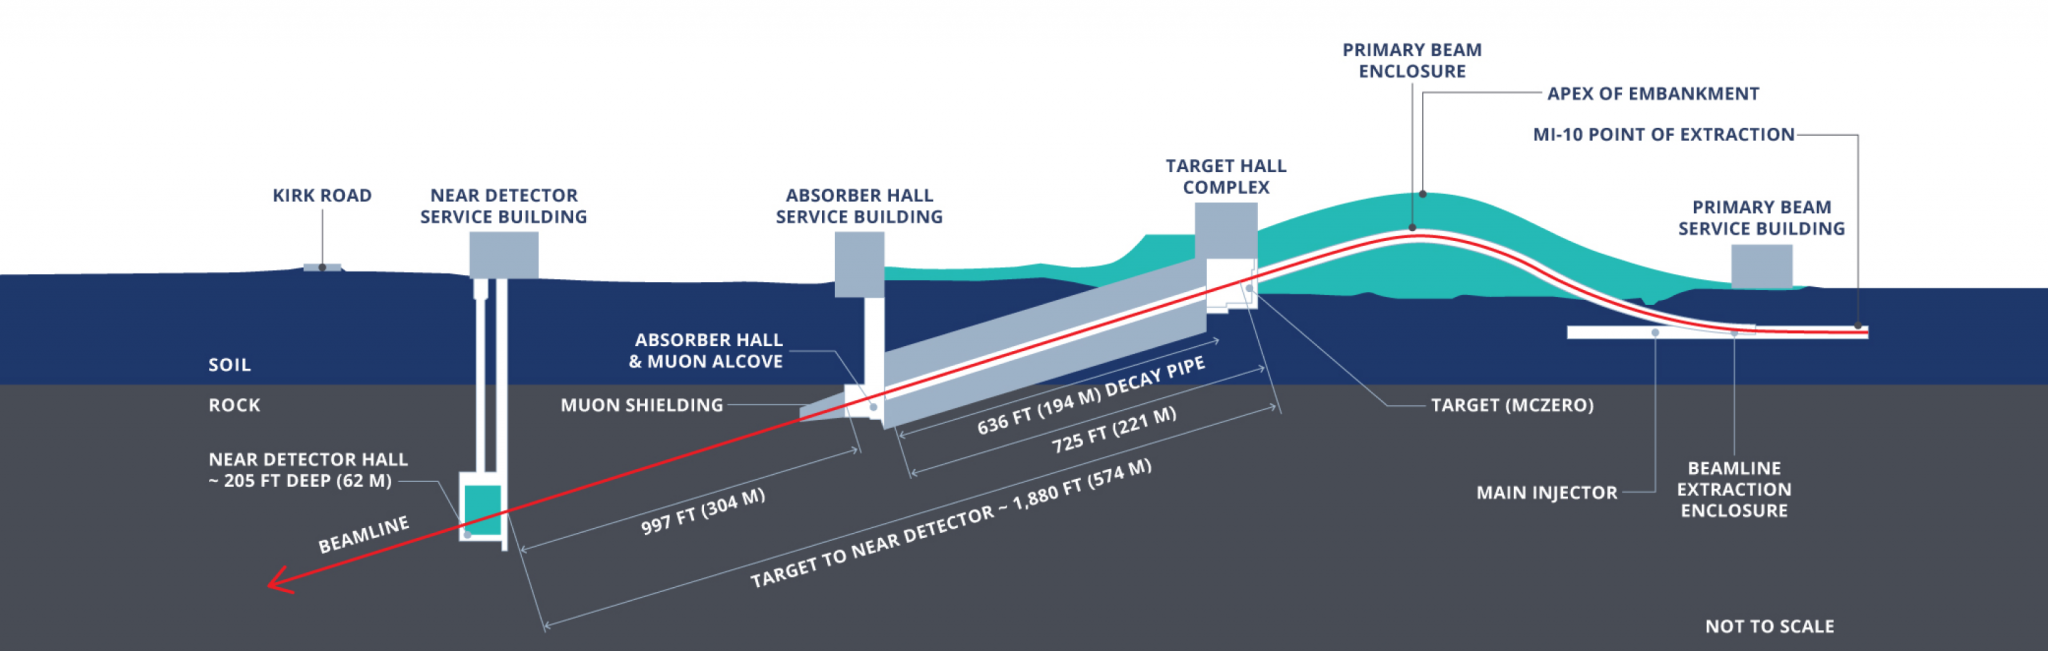
\includegraphics[width=0.99\textwidth]{figures/ch3-DUNE/LBNF-IL-graphic-Fermilab-LBNF.png}
     \caption[Longitudinal section of the LBNF beamline facility at Fermilab]{Longitudinal section of the LBNF beamline facility at Fermilab. The beam comes from the right, the protons being extracted from the main injector \cite{LBNFpage}. }
        \label{fig:LBNFgrafics}
\end{figure}
The DUNE experiment's neutrino flux will be produced by the LBNF beamline at Fermilab, which is expected to produce the highest power neutrino beam in the world \cite{DUNE:2016LBNFTDR, Papadimitriou:2016ksv}. The production of the neutrino flux begins by accelerating protons through a proton accelerator (see Fig. \ref{fig:LBNFgrafics} for a schematic representation). The primary proton beam, which operates in the energy range of 60-120 GeV, is extracted from Fermilab's main injector (MI), a proton accelerator already utilized by the NOvA experiment and partially based on the Tevatron collider facilities. The main injector will be upgraded through the Proton Improvement Plan, phase II (PIP-II), in time for the DUNE Phase I data taking period to reach average beam powers of the order of 1.14 MW, delivering $7.5 \times 10^{13}$ protons in one MI machine cycle (0.7 sec - 1.2 sec) to the LBNF target. Further improvements are expected the PIP III project to reach 2.4 MW of power for DUNE Phase II and all the beamline components are being planned to accommodate these improvements with minimal retro-fitting. 

Once the primary proton beam reaches the desired energy, it is directed through the use of extraction and transport components over a man-made hill and bent downwards towards a graphite target located at grade level. This constitutes the first element of the proper neutrino beamline. The charged mesons, primarily kaons and pions, produced in the interactions of the protons are sign selected and focused by two magnetic horns into a decay pipe toward the far detector. The target and focusing horns are all located inside a heavily shielded vault called the target chase, that is isolated from the decay pipe at its downstream end by a metallic window. Their design is derived from that of the NuMi neutrino beam. 

The mesons produced in the proton interactions are short-lived and decay into either anti-muons and neutrinos or muons and anti-neutrinos, depending on the charge of the mesons. If the main neutrino types being produced are $\nu_\mu$ the beamline is said to be in forward horn current (FHC) mode, otherwise it is said to be in reverse horn current (RHC) mode.  Both polarities will produce high purity fluxes, with an expected contamination from the “incorrect” neutrino type (i.e. $\nu_\mu$ in RHC mode and vice-versa) of less than 10\% in the oscillation energy region. This type of impurities are introduced by hadrons of the opposite sign propagating at the centre of the beam, where no magnetic field is present. A small $\nu_e$ and $\Bar{\nu}_e$ component is also introduced by the decay of secondary kaons and tertiary muons from pion decays. At the end of the decay region, an absorber is needed to remove the residual hadrons remaining at the end of the decay pipe.  The absorber core consists of replaceable aluminium and steel water-cooled blocks. Approximately 40\% of the beam power is deposited in the target chase and surrounding shielding, 30\% in the decay pipe and 30\% in the absorber.

The wide band neutrino beam which is produced by the beamline facilities, is needed to cover the first and second neutrino oscillation maxima, which for a 1300 km baseline are expected to be approximately at 2.4 and 0.8 GeV. For this reason the beamline design is optimized for neutrino energies between 0.5 and 5 GeV. 

\subsection{The far detector}
\begin{figure}[!ht]
     \centering
     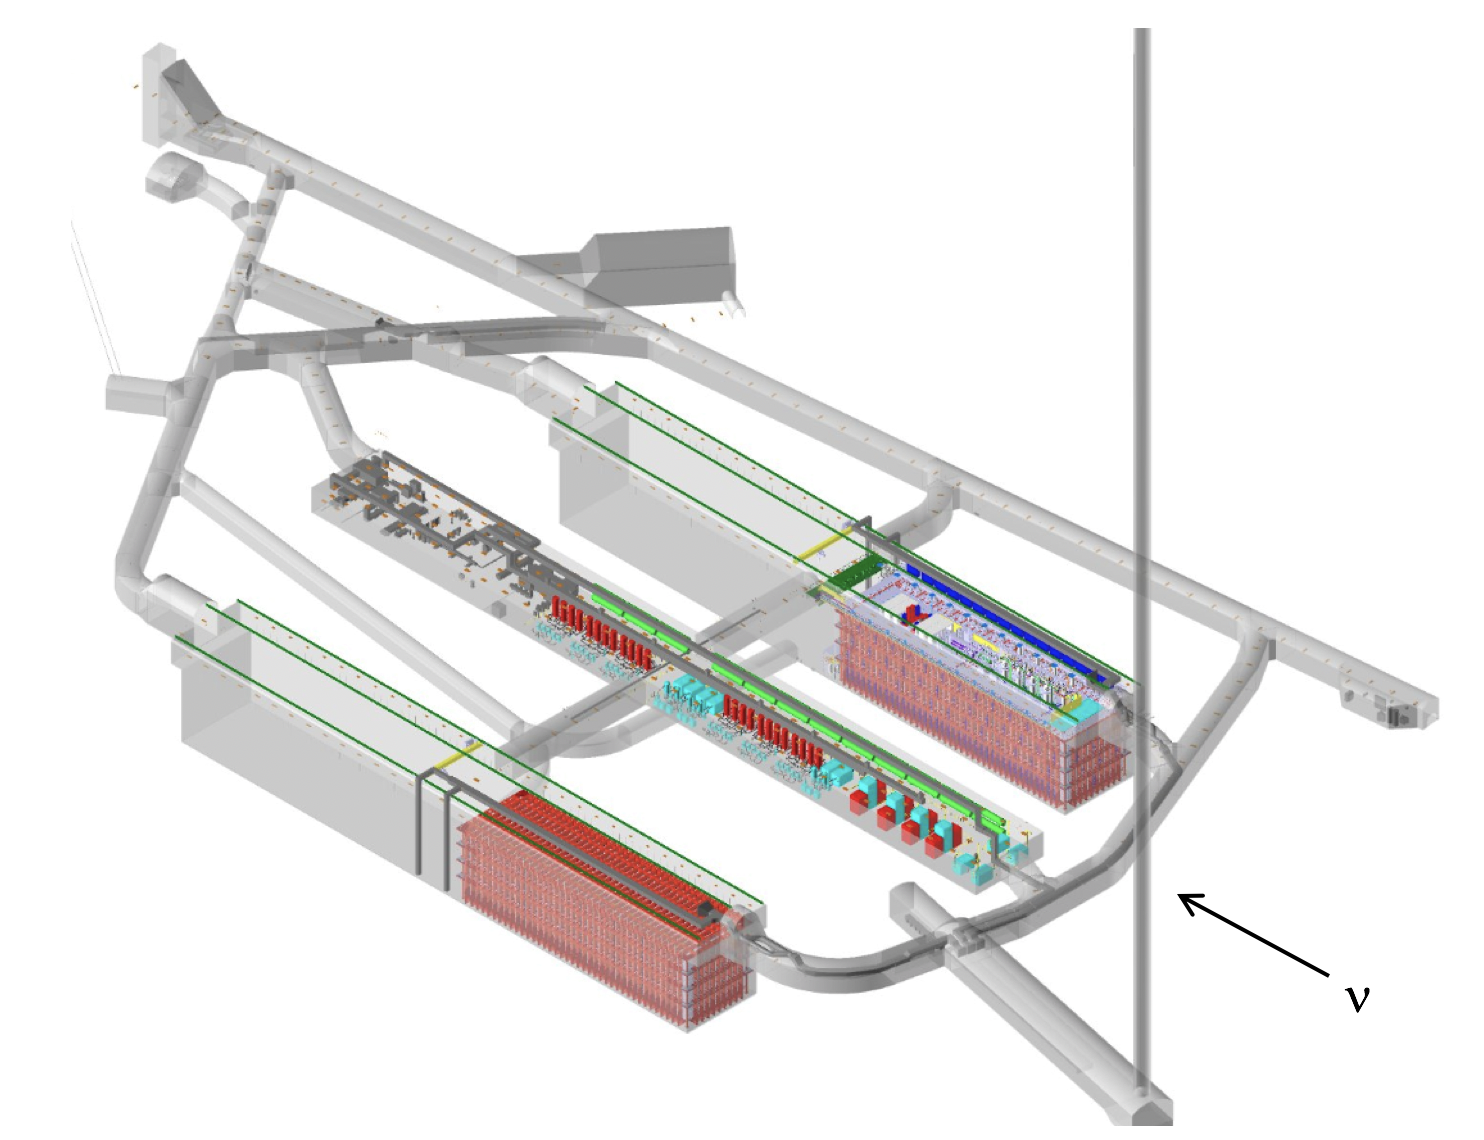
\includegraphics[width=0.7\textwidth]{figures/ch3-DUNE/caverns_full_assembly.png}
     \caption[Underground caverns for DUNE FD and cryogenics systems at SURF, in South Dakota.]{Underground caverns for DUNE FD and cryogenics systems at SURF, in South Dakota. The drawing, which looks towards the northeast, shows the first two far detector modules in place. \cite{DUNE:2020ypp}.}
        \label{fig:FarDetectorHall}
\end{figure}
The DUNE FD will be composed of four LArTPC detector module, each containing a 10kt fiducial liquid Argon mass  and a total liquid Argon mass of 17.5kt. Each module will fit inside a cryostat. Of the four modules only the first two will be available during DUNE Phase I, the first one using an horizontal drift technology (originally identified as single phase (SP) \cite{DUNE:2020TDR4}) will be called FD1-HD and the second one using a vertical drift technology\cite{DUNE:2023TDRVD} (evolved from the dual phase (DP) technology \cite{DUNE:2018mlo}) will be called FD2-VD. The last two modules will be employed during Phase II and are nominally set to be VD detectors\cite{DUNE:2022Snowmass}.

The LArTPC was pioneered by the ICARUS experiment \cite{Rubbia:1977zz,ICARUS:2004wqc} and is now a mature detector technology within the neutrino experiment community, being employed in detectors such as MicroBooNe\cite{MicroBooNE:2016pwy} and SBND\cite{Machado:2019oxb} at Fermilab as well as the ProtoDUNE-SP\cite{DUNE:2020cqd} prototype tested at the CERN neutrino facilities. In a LArTPC, ionization electrons produced by the energy deposition of charged particles generated in neutrino interactions, are drifted by an electric field in the liquid Argon towards an anode and are collected on a charge multiplier element, producing a readable two dimensional signal. The measurement of the collected ionization electrons also provides a measurement of the $dE/dx$ of the charged particles, which is what enables both calorimetry and particle identification (PID) in a LArTPC.

Argon is a UV light scintillator. Once shifted into the visible spectrum, the UV scintillation photons produced by can be collected by photon detectors and provide an initial start time $t_0$, indicating when the ionization electrons begin to drift. Comparing the time at which the ionization signal reaches the anode relative to this start time allows reconstruction of the event topology in the drift coordinate. For a simple visualization of the LArTPC technique see Fig. \ref{fig:LArTPCdiagram}.

The FD1-HD design combines a kt level fiducial mass with a sub-cm spacial resolution. Both are crucial to achieve DUNE's scientific goals of measuring CP violation, while searching for nucleon decay and being capable of observing neutrinos from supernova bursts. An example of the design of the detector being directly informed by the physics requirements of the experiment, comes from the electron/photon separation requirements necessary to study $\nu_e$ appearance signals in the LBNF $\nu_\mu$ flux. Electrons are typically produced in charged current $\nu_e$ interactions and induce electro-magnetic showers in the LAr medium. Similar electro-magnetic activity can be induced by photons coming for example from $\pi^0$ decay. The FD modules are capable of distinguishing between these two signals by using $dE/dx$ information combined with spacial information. Photon induced signals have an initial non ionized gap of several cm's before the formation of the electro-magnetic shower and have an initial $dE/dx$ which is double that of an electron induced one.

The FD1-HD detector modules consist of 4 separate liquid Argon drift volumes with a maximum drift length of 3.5 m. Each volume is instrumented with a vertical cathode plane and an anode plane, for a total of three module-long (58.2 m) anode planes and two cathode planes. A field cage covers the spaces between the two, producing a stable 500 V/m electric field in the horizontal direction. The drift ionization electrons reach the anode planes in an order of a few milli-seconds. 

Each anode plane is instrumented with a total of 50 anode plane assemblies APAs which consist of an aluminum frame with three layers of active wires and an additional shielding layer wrapped around them. The first two active layers are identified as the U and V induction layers. These layers are angled at a $\pm 37.5^\circ$ in order to reduce ambiguities in event reconstruction. The relative voltage between the layers is chosen so that the drift electrons pass through them and produce a bipolar induction signal on both planes. The drifting electrons are finally collected in the final $X$ wire plane, where they produce a mono-polar signal. In the $X$ collection plane, as well as in the $G$ shielding plane, the wires run vertically. The spacing between the wires in each layer is of 5 mm, and defines the spacial resolution of the APAs.

The scintillation photons produced by the passing charged particles in the liquid Argon in the very ultra violet (VUV) spectrum are collected by photon detector (PD) systems called X-ARAPUCA \cite{Segreto:2018jdx}. The photons are produce in the order of 24000 per MeV of deposited energy, and reach the detectors in a time-frame of the order of a nanosecond. The X-ARAPUCA modules are mounted between the sets of wire-planes and consist of layers of dichroic filter and wavelength shifters, that shift the VUV scintillation light into the visible range, trap the visible photons, and transport them to a silicon photo-multiplier (SiPM). The signals produced in the SiPMs are then combined with the wire signals from the APAs at the data acquisition (DAQ) level.

\begin{figure}[!t]
     \centering
     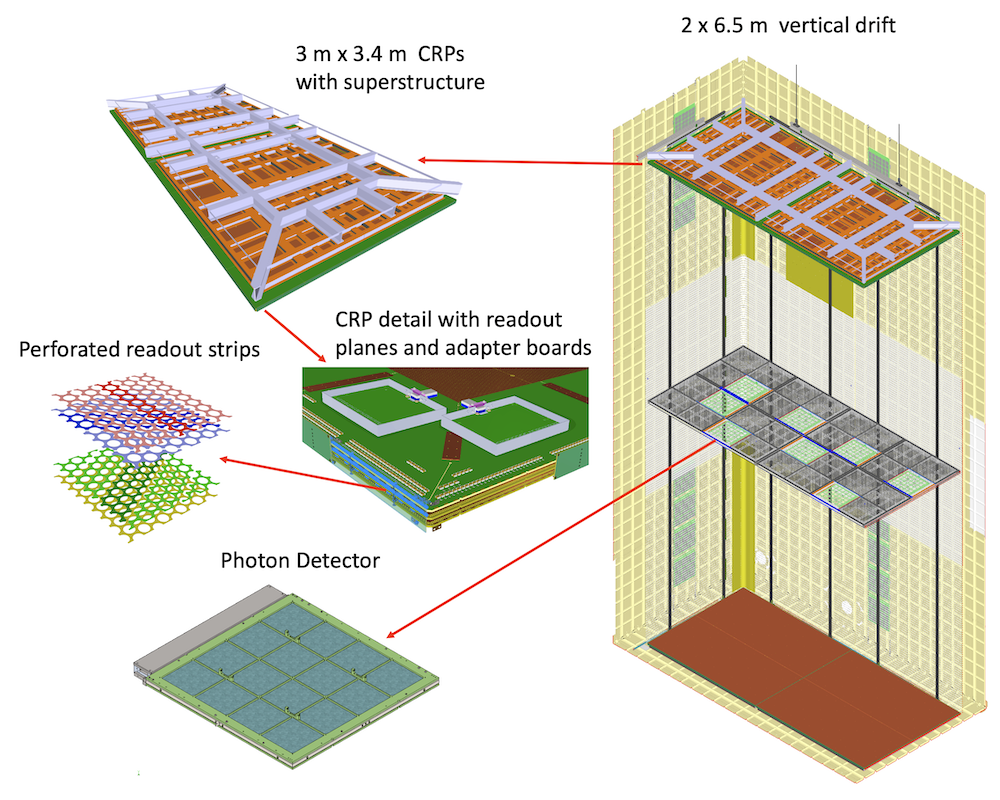
\includegraphics[width=0.7\textwidth]{figures/ch3-DUNE/setup_new_updated.png}
     \caption[Schematic view of a vertical drift module concept with PCB-based charge readout.]{Schematic view of a vertical drift module concept with PCB-based charge readout. Corrugations on cryostat wall shown in yellow; PCB-based CRPs (brown, at top and bottom with superstructure in gray or top CRPs); cathode (violet, at mid-height with openings for photon detectors); field cage modules (white) hung vertically around perimeter (70\% transparent portion in regions near anode planes); photon detectors, placed in the openings on the cathode and on the cryostat walls, around the perimeter in the vertical regions near the anode planes. \cite{DUNE:2023TDRVD}.}
        \label{fig:FDLArTPCModule}
\end{figure}

The FD2-VD design was developed from the R\&D experience accumulated by the DUNE collaboration with the ProtoDUNE-SP and ProtoDUNE-DP prototypes at the neutrino research facilities at CERN \cite{DUNE:2023TDRVD}. The detector consists of several vertical drift modules enclosed in a large cryostat structure. Each module is divided into two vertical drift regions 6.5 m in height by an horizontal cathode, and feature two anode planes, one close to the cryostat top, just below the surface of the liquid Argon region and one close to the bottom of the cryostat. Field cage modules hang vertically around the module's perimeter. The 450 V/cm electric field drifts the ionisation electrons, either upwards or downwards depending on the drift region. The vertical design of the FD2-VD offers a slightly larger instrumented module compared to FD1-HD and it's more cost-effective thanks to its high-modularity and general structure and geometry. 

The anode planes in the FD2-VD design consist of two double-sided perforated printed circuit boards (PCB's) that are connected to form a charge-readout unit (CRU's). The perforation holes allow the electrons to pass through the PCB's. The first PCB is instrumented with two sets of induction strips, while the second one hosts the collection strips. The three planes of strips are segmented at about 7.5 mm pitch for the induction planes and 5 mm pitch for the collection plane, and are set at $60^\circ$ angles relative to each other to maximize information in the charge readout from different projections. Two CRU's are connected to a frame to form a Charge Readout Plane (CRP). Each anode plane consists of 80 CRP's. Much like in the FD1-HD design the anode plane signal allows for a two-dimensional reconstruction of any given event, while the third dimension is given by the drift time information obtained from the scintillation light.

The photo-detectors implemented in the FD2-VD follow the same general design of the ARAPUCA-X modules developed for FD1-HD. The PD's will be mounted on the four cryostat membrane walls as on both sides of the central cathode structure. This configuration offers a uniform ligth measurement coverage across the entire LArTPC volume. Additionally, the FD2-VD liquid argon will be doped with a small quantity of xenon. This has no impact on the TPC operation but significantly enhances the photon detection performance. A schematic representation of the vertical drift modules' design is shown in Fig. \ref{fig:FDLArTPCModule}.

\subsection{The near detector}
\label{Sec:Near}

\begin{figure}[!h]
     \centering
     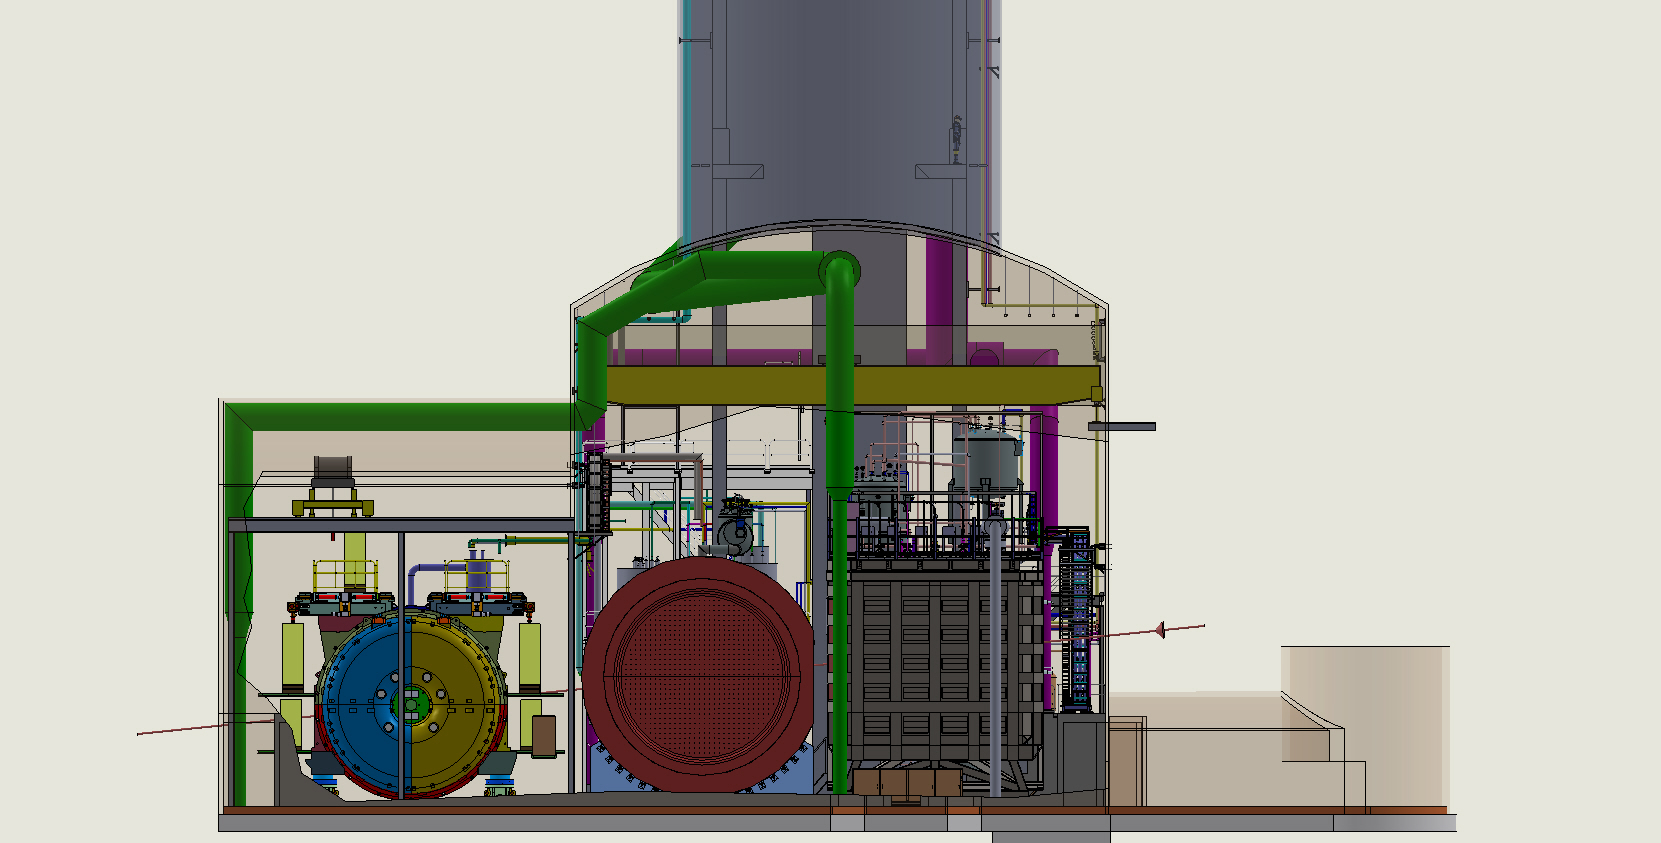
\includegraphics[width=0.99\textwidth]{figures/ch3-DUNE/ndhall.JPG}
     \caption[Schematic side-view of DUNE's ND hall.]{Schematic side-view of DUNE's ND hall. The neutrino beam direction is given roughly by the red arrow and from right to left the detectors ND-LAr, ND-GAr and SAND are shown \cite{Battisti:2022ND}.}
        \label{fig:NDhall}
\end{figure}

To enable oscillation measurements, DUNE must first predict the anticipated signal and background at the FD based on oscillation parameters, followed by a comparison with measured flavour-tagged neutrino spectra. To generate this prediction, one must determine the neutrino flux at production, neutrino interaction cross-sections, and detector response—factors all affected by systematic uncertainties requiring constraint (see Sec. \ref{Sec:NDScientific} for a more detailed discussion). The near detector is tailored to address each prediction component \cite{DUNE:2021NDCDR}: it will gauge the un-oscillated neutrino beam flux both on-axis and at varying off-axis angles; refine models of neutrino interactions through cross-section and final state topology measurements; model detector responses relative to neutrino energy. Additionally, the ND is designed for operation within a high event rate environment, ensuring the requisite statistical coverage across the full phase-space. The ND will consist of three detectors with complementary designs: ND-LAr, which will use a LArTPC technology similar to the FD modules; ND-GAr, a gaseous Argon TPC detector; and SAND, a magnetized beam monitor. ND-LAr and ND-GAr are movable off-axis, while SAND remains fixed on-axis. A schematic depiction of the ND, inclusive of all detectors, is presented in Figure \ref{fig:NDhall}. Due to budgetary reasons the ND-GAr detector will become available only during Phase II of the DUNE experiment. A much simpler detector referred to as the temporary muon spectrometer (TMS) will replace it during Phase I. 

\begin{figure}[!t]
     \centering
     \begin{subfigure}[b]{0.59\textwidth}
         \centering
         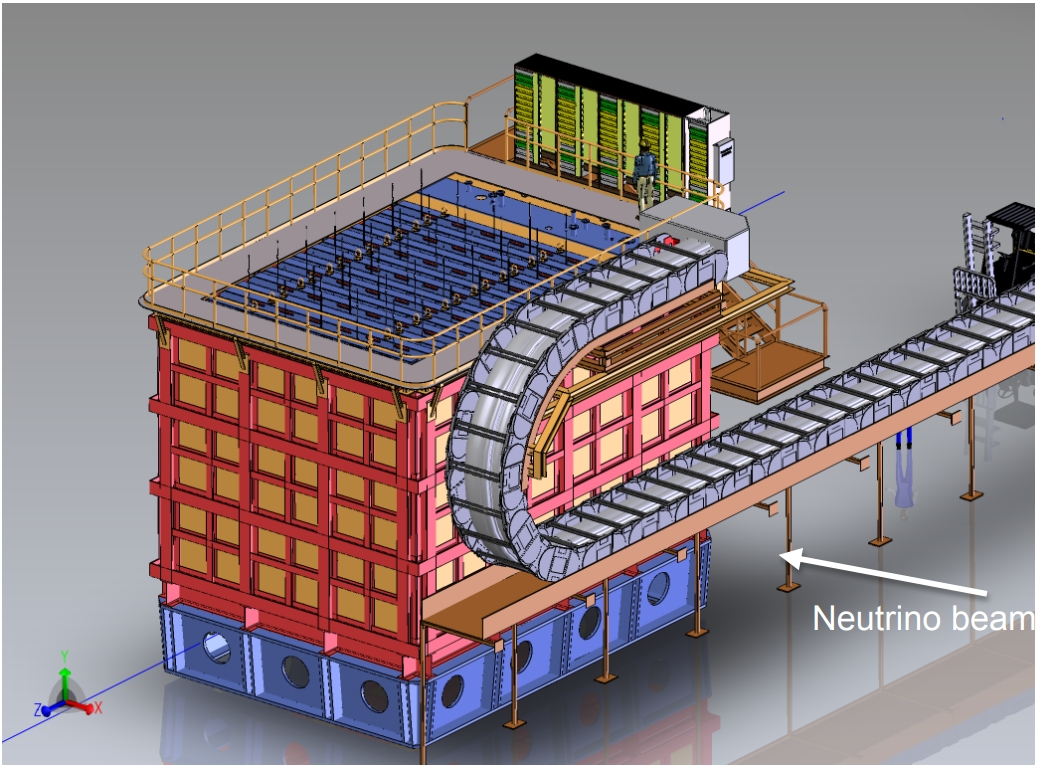
\includegraphics[width=\textwidth]{figures/ch3-DUNE/ND-LAr.jpg}
         \caption{}
         \label{fig:NDLAr}
     \end{subfigure}
     \begin{subfigure}[b]{0.39\textwidth}
         \centering
         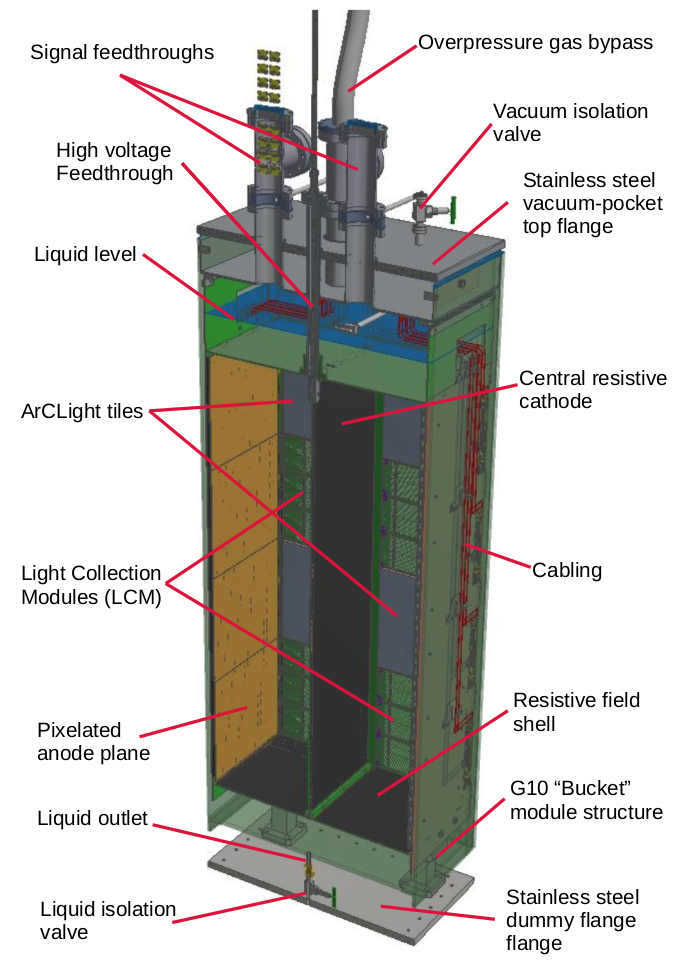
\includegraphics[width=\textwidth]{figures/ch3-DUNE/ND-LAr_module.png}
         \caption{}
         \label{fig:NDLArModule}
     \end{subfigure}
        \caption[Schematic view of ND-LAr.]{(Left) Schematic view of the external components of ND-LAr, including the cryostat and the system for the DUNE-PRISM movement (Right) Schematic drawing of a single ND-LAr module with its major components individually highlighted \cite{Battisti:2022ND}.}
        \label{fig:ND-Larview}
\end{figure}

ND-LAr will be a LArTPC detector engineered for operation within a high-rate environment. Utilizing the same Argon target and similar detector technology as the FD modules, ND-LAr is essential for modeling detector response and liquid Argon neutrino interaction cross-sections. ND-LAr is comprised of 35 distinct TPC modules, mirroring the design of the ArgonCube prototype \cite{Dwyer:2018phu}. Despite the relativly modest dimensions of the detector, this modular architecture is indispensable for managing the high event rate, facilitating a smaller drift region, enhanced light separation, and increased sensor pixelation. Each module encompasses two optically isolated TPCs outfitted with a LArPix-based pixelated charge readout system  \cite{Goldi:2018mbo}, alongside a light readout for rapid timing data from prompt scintillation light, and a field structure ensuring minimal field non-uniformity throughout the active volume. Given the relatively compact dimensions of its active volume, ND-LAr cannot fully contain the majority of muons generated in $\nu_\mu$ Charged Current (CC) interactions within liquid Argon. Hence, precise momentum reconstruction of this muon sample necessitates an external spectrometer component, a role fulfilled by ND-GAr and the TMS.

\begin{figure}[t]
     \centering
     \begin{subfigure}[b]{0.5\textwidth}
         \centering
         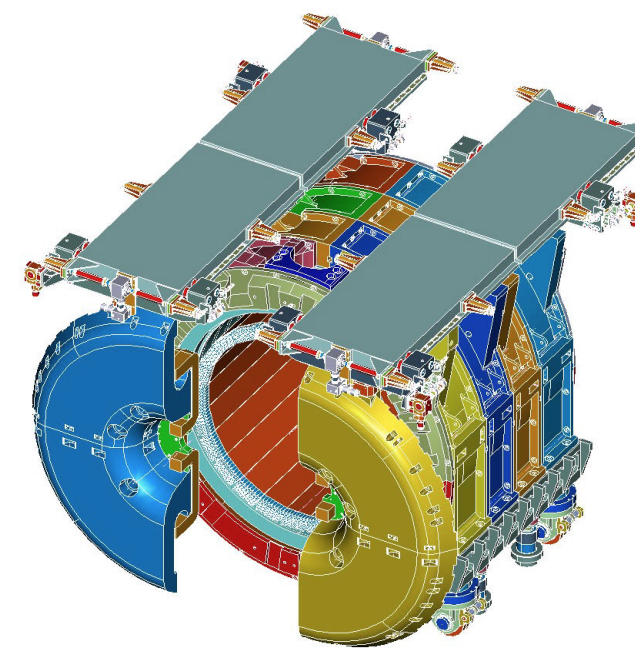
\includegraphics[width=\textwidth]{figures/ch3-DUNE/SAND.png}
         \caption{}
         \label{fig:SAND-outside}
     \end{subfigure}
     \hfill
     \begin{subfigure}[b]{0.48\textwidth}
         \centering
         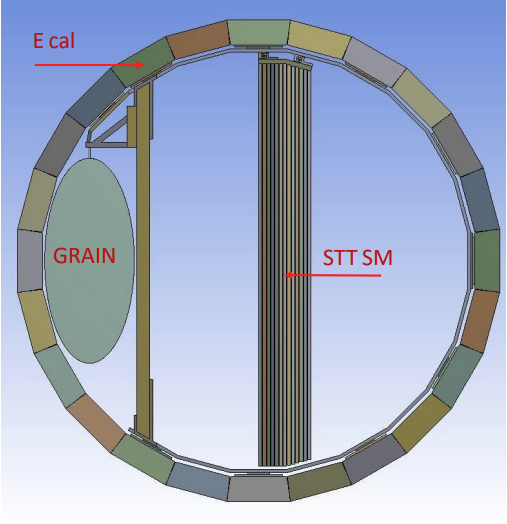
\includegraphics[width=\textwidth]{figures/ch3-DUNE/SAND-inside.png}
         \caption{}
         \label{fig:SAND-inside}
     \end{subfigure}
        \caption[Schematic view of SAND.]{(Left) Schematic view of the external components of SAND, including its cryostat and its solenoid magnet (Right) Side view of the internal components of SAND, including its active liquid Argon target called GRAIN, one of the straw tube tracker modules and the electro-magnetic calorimeter \cite{Battisti:2022ND}.  }
        \label{fig:SAND-all}
\end{figure}

ND-LAr and ND-GAr possess the capability to be translated up to 30 meters perpendicular to the neutrino beam axis, spanning angles from $0^{\circ}$ to $3^{\circ}$, a feature named DUNE precision reaction independent spectrum measurement (PRISM). With increasing off-axis angles, the mean energy of the neutrino flux diminishes while its energy dispersion narrows. Consequently, the ND gains access to diverse un-oscillated neutrino flux profiles, which can be combined to predict the oscillated flux at the far detector. This data-centric methodology mitigates reliance on models. Moreover, a key feature of the DUNE-PRISM program is that the off-axis fluxes will variate in mean energies and spreads and will thus be dominated by distinct interaction types (e.g. quasi-elastic, resonant etc.). Access to this variety of samples will facilitate the disentanglement of cross-section effects, enhancing flux and interaction modeling.

The system for on-axis neutrino detection (SAND) will function as a constant on-axis monitor of the neutrino beam, a crucial role for the DUNE-PRISM program. It will ensure that any differences in flux measured by ND-LAr and ND-GAr result from their off-axis position rather than anomalies in beam production. SAND's main structural components, along with its solenoid magnet, cryostat, and electromagnetic calorimeter, will be repurposed from the KLOE experiment (Figure \ref{fig:SAND-all}). The internal tracker design of SAND has recently been finalized, featuring a Straw Tube Tracker (STT) divided in modules \cite{Battisti:2022ND}. These modules will include a series of tunable passive slabs interleaved with tracking layers of 5mm diameter tubes. SAND will provide various targets, such as CH$_2$ and C, potentially highly useful in studying neutrino interactions. They will offer a clean sample of neutrino-on-hydrogen interactions by "subtraction" devoid of nuclear effects. Additionally, SAND will incorporate its own active target of liquid Argon called granular Argon for interaction of neutrinos (GRAIN), whose design is currently being finalized. 

\section{The ND-GAr detector}
\label{sec:DUNE-ND-GAr}

\begin{figure}[t]
     \centering
     \includegraphics[width=0.6\textwidth]{figures/ch3-DUNE/SPY_X-section2.jpg}
     \caption[Cut-away view showing the various components of ND-GAr.]{Cut-away view showing the various components of ND-GAr \cite{Bersani:2023rlw}.}
        \label{fig:ND-G}
\end{figure}

ND-GAr will be a magnetized detector with a magnetic field of 0.5T, mainly constituted of a high pressure gas time projection chamber (HPgTPC) surrounded by an electro-magnetic calorimeter (ECAL). A simple cut-away schematic of the detector is shown in Figure \ref{fig:ND-G}. ND-GAr will fulfill two main goals: firstly it will act as a spectrometer measuring the charge and momentum of particles exiting ND-LAr; secondly it will offer its own sample of neutrino interactions inside the HPgTPC. The high pressure gas environment will offer relatively low tracking thresholds and enhanced particle identification performance when compared to LArTPC's, especially for pion-proton separation. The PID capabilities of ND-GAr specifically derive from a combination of $dE/dx$ measurements in the HPgTPC, $E/p$ measurements in the ECAL and the curvature momentum and sign selection measurements available from the magnetization of the TPC alongside range measurements in the ECAL.

ND-GAr's spectrometer role mostly consists in identifying the sign and measuring the momentum of muons exciting ND-LAr. This is done to measure the spectrum of $\nu_\mu$ and $\Bar{\nu}_\mu$ reaching the near detector, through their CC interaction products. This is crucial to reach the oscillation measurement sensitivity desired by the experiment.

\begin{figure}[t]
     \centering
     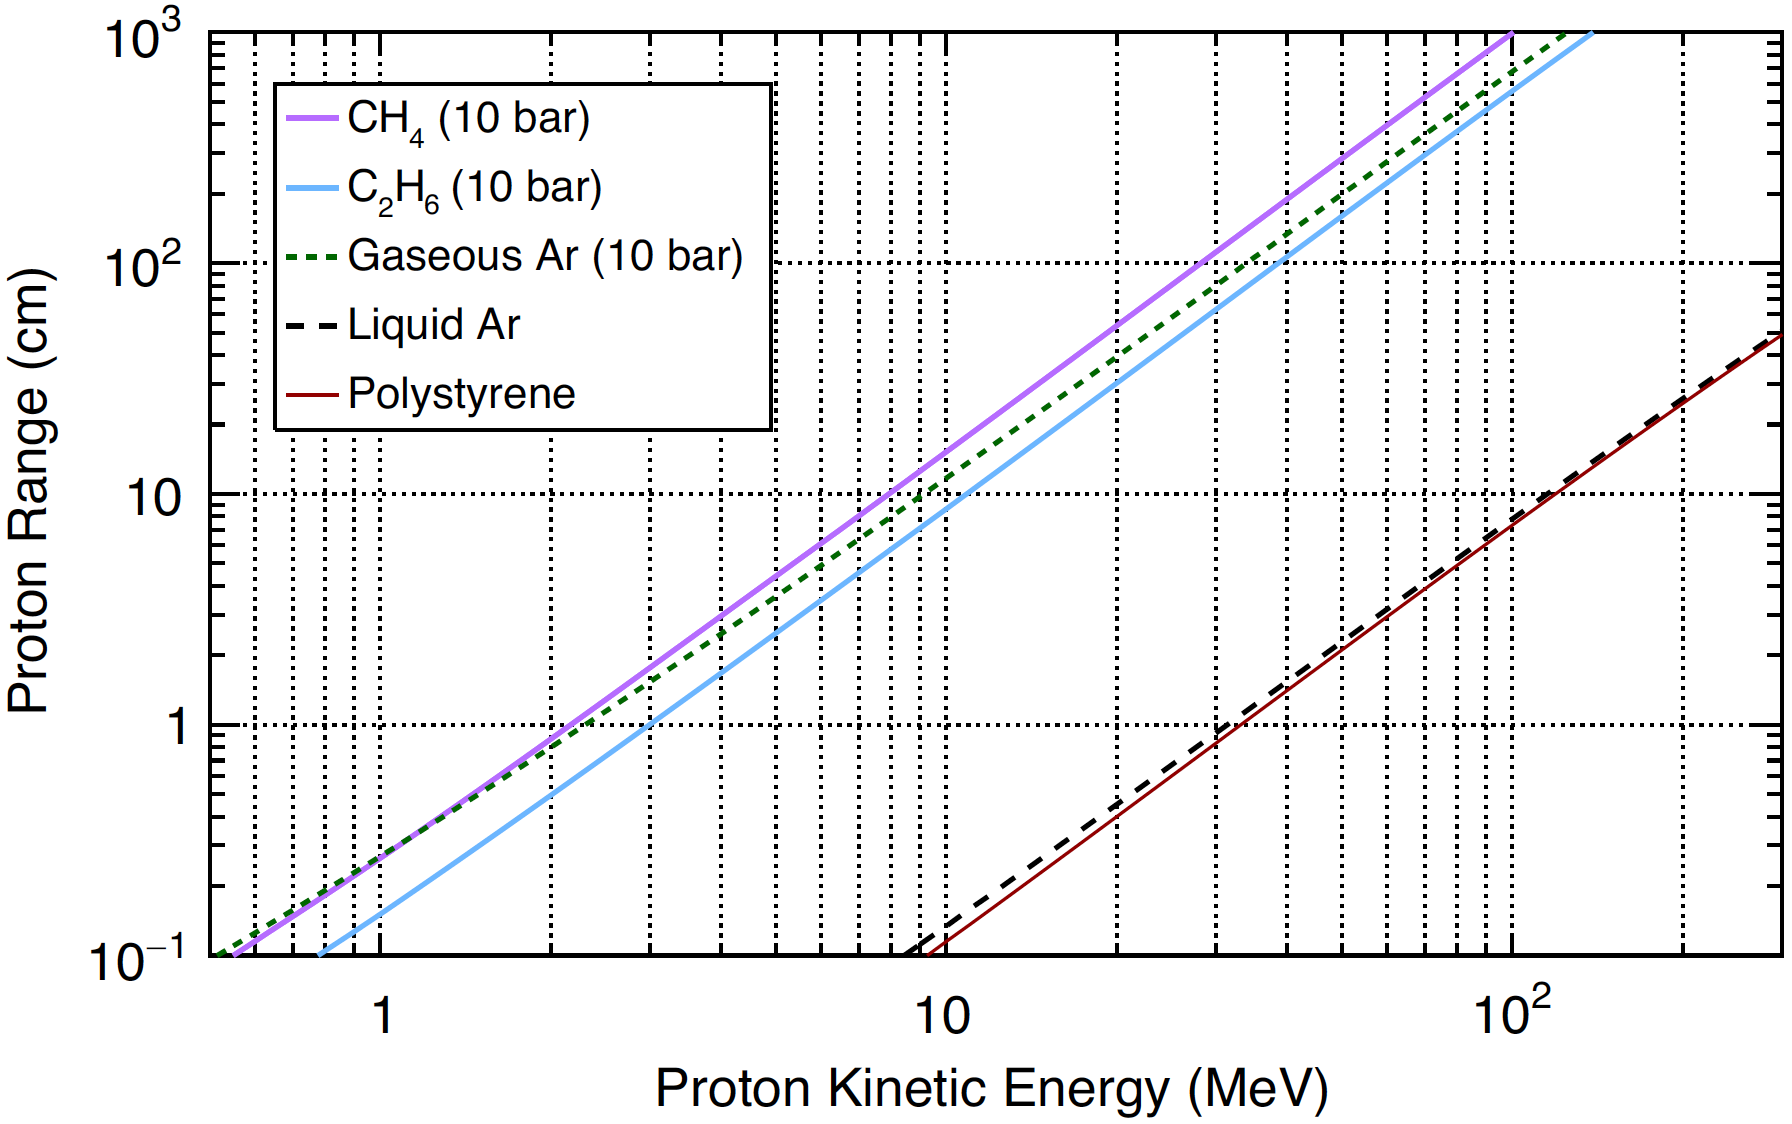
\includegraphics[width=0.7\textwidth]{figures/ch3-DUNE/threshold.png}
     \caption[Plot showing proton range in cm as a function of kinetic energy.]{Plot showing proton range in cm as a function of kinetic energy in MeV in double logarithmic scale. The different curves show the range dependency in different gaseous, liquid or solid media \cite{Lu}.}
        \label{fig:ND-G-threshold}
\end{figure}

ND-GAr's lower tracking thresholds as well as its superior PID capabilities and acceptance, will make kinematic regions not accessible to a LAr detector, available to the ND complex. The relationship between proton tracking threshold and tracking material can be seen in Figure \ref{fig:ND-G-threshold}. This is particularly important to enhance the ability of the ND of clarifying the relationship between the true and reconstructed energy in neutrino interactions on Argon. Nuclear effects such as final state interactions, Fermi motion and 2p2h effects can introduce significant systematic uncertainties in the reconstruction of the neutrino energy. Theoretical studies suggest for example that FSI can increase dramatically the number of final state protons in the kinetic range of 10s of MeV's and it's thus crutial for the ND to be able to measure them and identify them. This is possible with a HpGTPC which has lower tracking thresholds, but not in a LAr or solid detector such as ND-LAr or SAND. 

It is also important for ND-GAr to characterize the spectrum of charged pions coming from $\nu_\mu$ and $\Bar{\nu}_\mu$ CC interactions. At very low energies, down to 20 MeV , this is essential because this is the region where FSI's are more prevalent. Only a gaseous detector has low enough energy thresholds to do it with a sufficient efficiency. At higher energies above 100 MeV, ND-GAr becomes essential in distinguishing the pion multiplicity, since in LAr the same pions tend to produce hadronic showers, while in ND-GAr's TPC they are more likely to produce distinguishable tracks. Measuring neutral pions from $\nu_\mu$ and $\Bar{\nu}_\mu$ CC interactions in the same momentum range is also possible for ND-GAr thanks to its ECAL.

\subsection{The HpGTPC}
The design of ND-GAr's HPgTPC is closely related to the design of the ALICE experiment's TPC \cite{ALICE}. The basic detection mechanisms of ALICE's and ND-GAr's TPC's are identical. The primary ionization electrons are formed by the energy deposition of passing charged particles, and drifted towards the end-caps by a an electric field produced by a high voltage (HV) central electrode plane. The total drift region has a cylindrical shape with a diameter of $\sim 5 \ \text{m}$ and a length of $\sim 5 \ \text{m}$ and the electric field is oriented in parallel to the 0.5 T magnetic field, in order to reduce transverse diffusion. At the end-caps, multi-wire proportional chambers (MWPC's) induce electron avalanches which produce a signal on an anode pad plane. Read-outs of the pad signals give hit coordinates in two dimensions, while the drift time provides the third.

The read-out chambers or ROC's used in ALICE, contain the MWPC's and read-out pad planes and are divided in 18 trapezoidal regions, each including a smaller inner chamber (IROC) and an outer chamber (OROC). All of ALICE's ROC's will be re-installed in ND-GAr, as they have been replaced in the original detector by GEM-based ROC's \cite{Ferretti:2022yjd}. An additional central region of ROC's (CROC's) will fill the central regions of the read-out planes, which in ALICE was occupied by a silicon based central tracker and an inner field cage. 

Despite all the common elements, some key differences between the design of the two TPC's exist: the two detectors will use different gases, with ALICE's base gas being a mixture Ne/CO$_2$/N$_2$ and ND-GAr using a mixture of Ar-CH$_4$ at 90\%-10\% molar fractions; ND-GAr will operate at a pressure 10 times larger than ALICE; the electronics and data acquisition systems will be completely re-designed to be closer to the LArPix technologies used in DUNE's LArTPC's; the field cage will only include an outer component, since the central region in ND-GAr will be part of the active volume of the detector, while in ALICE it was occupied by the the beam pipe and a silicon-based tracker.
\begin{figure}[t]
     \centering
     \begin{subfigure}[b]{0.52\textwidth}
         \centering
         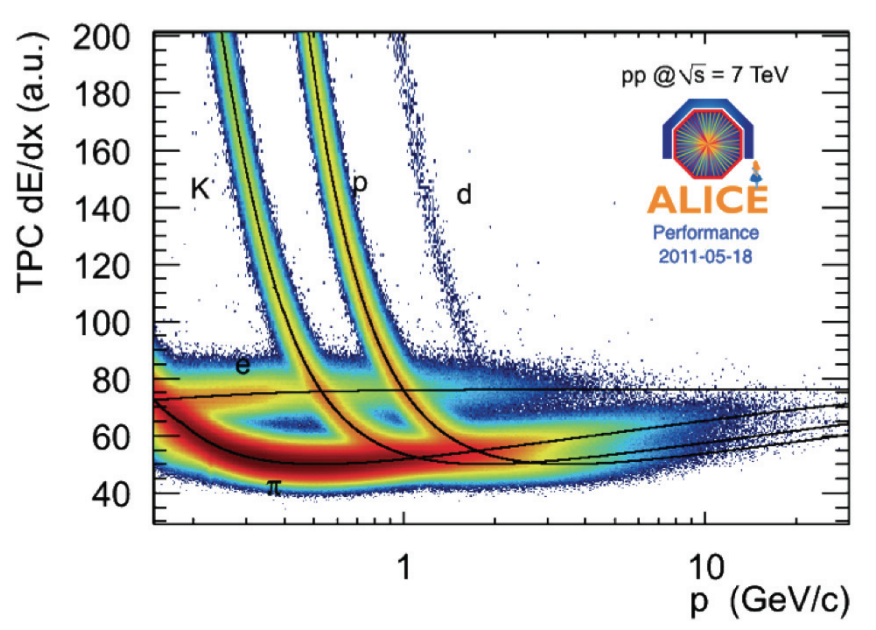
\includegraphics[width=\textwidth]{figures/ch3-DUNE/ALICE_TPC_dEdx_Lippmann_2012.png}
         \caption{}
         \label{fig:ALICEPID}
     \end{subfigure}
     \hfill
     \begin{subfigure}[b]{0.47\textwidth}
         \centering
         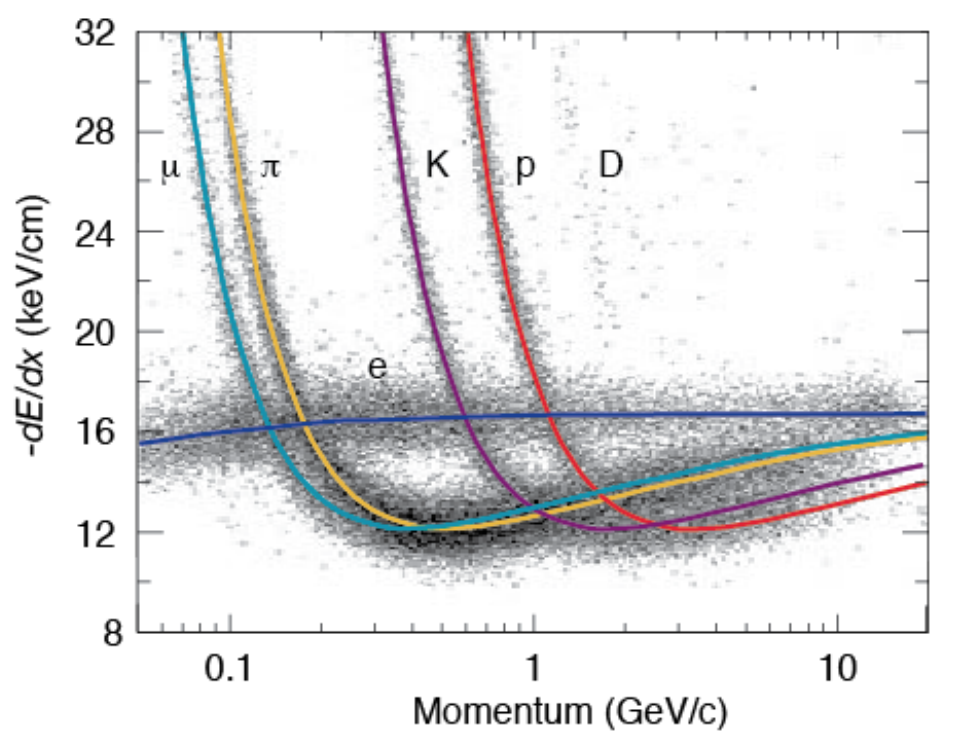
\includegraphics[width=\textwidth]{figures/ch3-DUNE/PEP4-TPC-80Ar-20CH4-8_5atm_dEdx.png}
         \caption{}
         \label{fig:PEPPID}
     \end{subfigure}
        \caption[ALICE and PEP-4/9 $dE/dx$ PID curves.]{(Left) ALICE TPC $dE/dx$-based particle identification as a function of momentum \cite{Lippmann:2012lwa}. (Right) PEP-4/9 TPC (80:20 Ar-CH4, operated at 8.5 Atm, from \cite{Grupen:1999by}) $dE/dx$-based particle identification. }
        \label{fig:PID}
\end{figure}

The HPgTPC is oriented so that the neutrino beam is perpendicular to the electric and magnetic fields. This is the most favorable orientation for measuring charged particles traveling along the neutrino beam direction. In ALICE the track reconstruction is done by combing ROC hits to form tracks following the trajectories of charged particles in the TPC. This is done for ND-GAr through the \texttt{GArSoft} software package which handles the simulation and reconstruction for the detector. A comprehensive description of this tool will be given later in Sec. \ref{Sec:GArSoft_Lite} and Sec. \ref{Sec:GArSoft-GAr} respectively. 

In ALICE the ionization induced by charged particle tracks can be used to estimate the particle's $dE/dx$. When combined with a curvature momentum estimate, this can be used for PID. In Fig. \ref{fig:ALICEPID} we show the characteristic PID curves for charged particles produced in proton-proton collisions at $\sqrt{s}=7 \ \text{TeV}$. The band resolution of the different particle types $dE/dx$ curves is expected to be significantly improved in ND-GAr. The 10 times higher gas pressure in ND-GAr will result in a correspondent increase in ionization per unit track length. A better comparison can be made with the performance of the PID capabilities of PEP-4/9, which operated at 8.5 atmospheres: the experiment's $dE/dx$ curves are plotted in Fig. \ref{fig:PEPPID} showing good separation between particle types below a few GeV, including pions and muons which are problematic for TPC's with lower material budgets. 

\begin{figure}[t]
     \centering
     \begin{subfigure}[b]{0.7\textwidth}
         \centering
         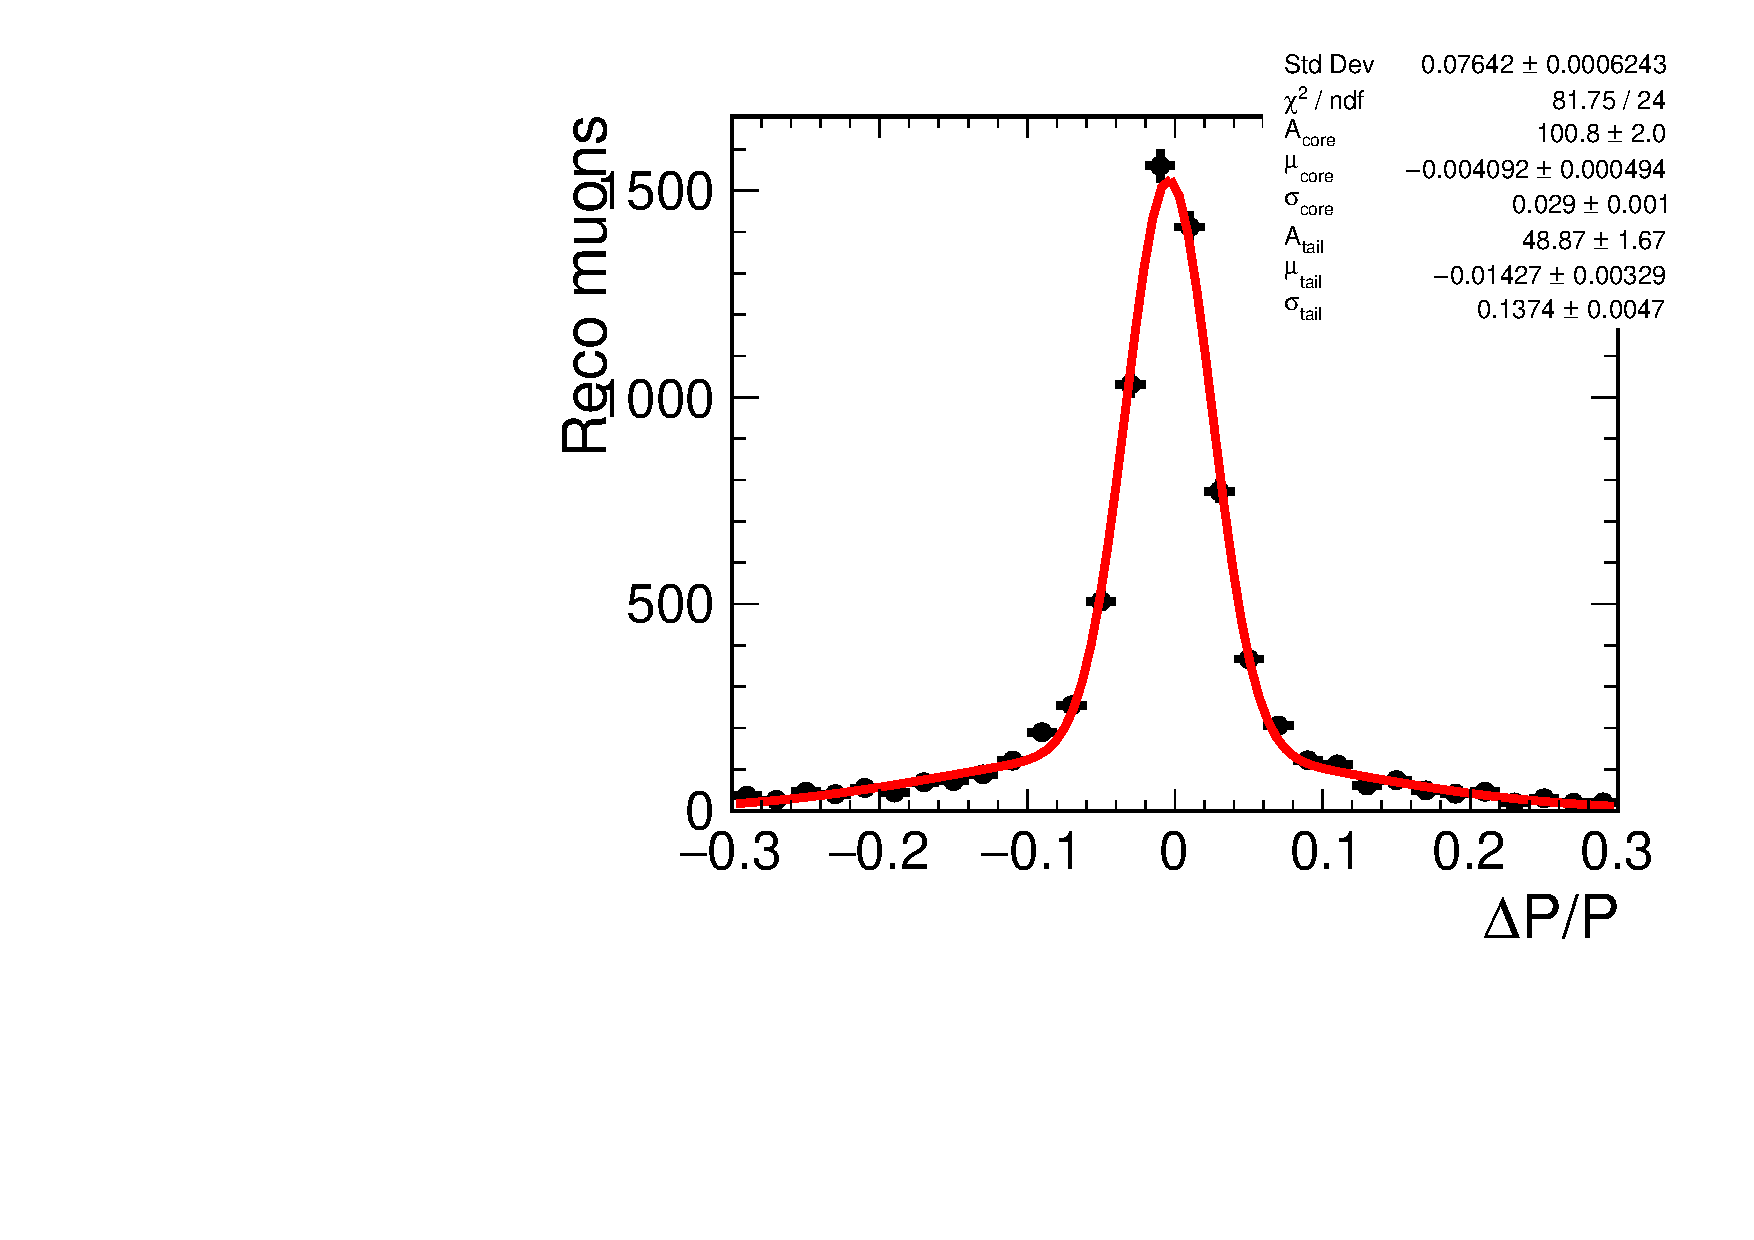
\includegraphics[width=\textwidth]{figures/ch3-DUNE/dpmuon.pdf}
         \caption{}
         \label{fig:GArTPCdp}
     \end{subfigure}
     \hfill
     \begin{subfigure}[b]{0.7\textwidth}
         \centering
         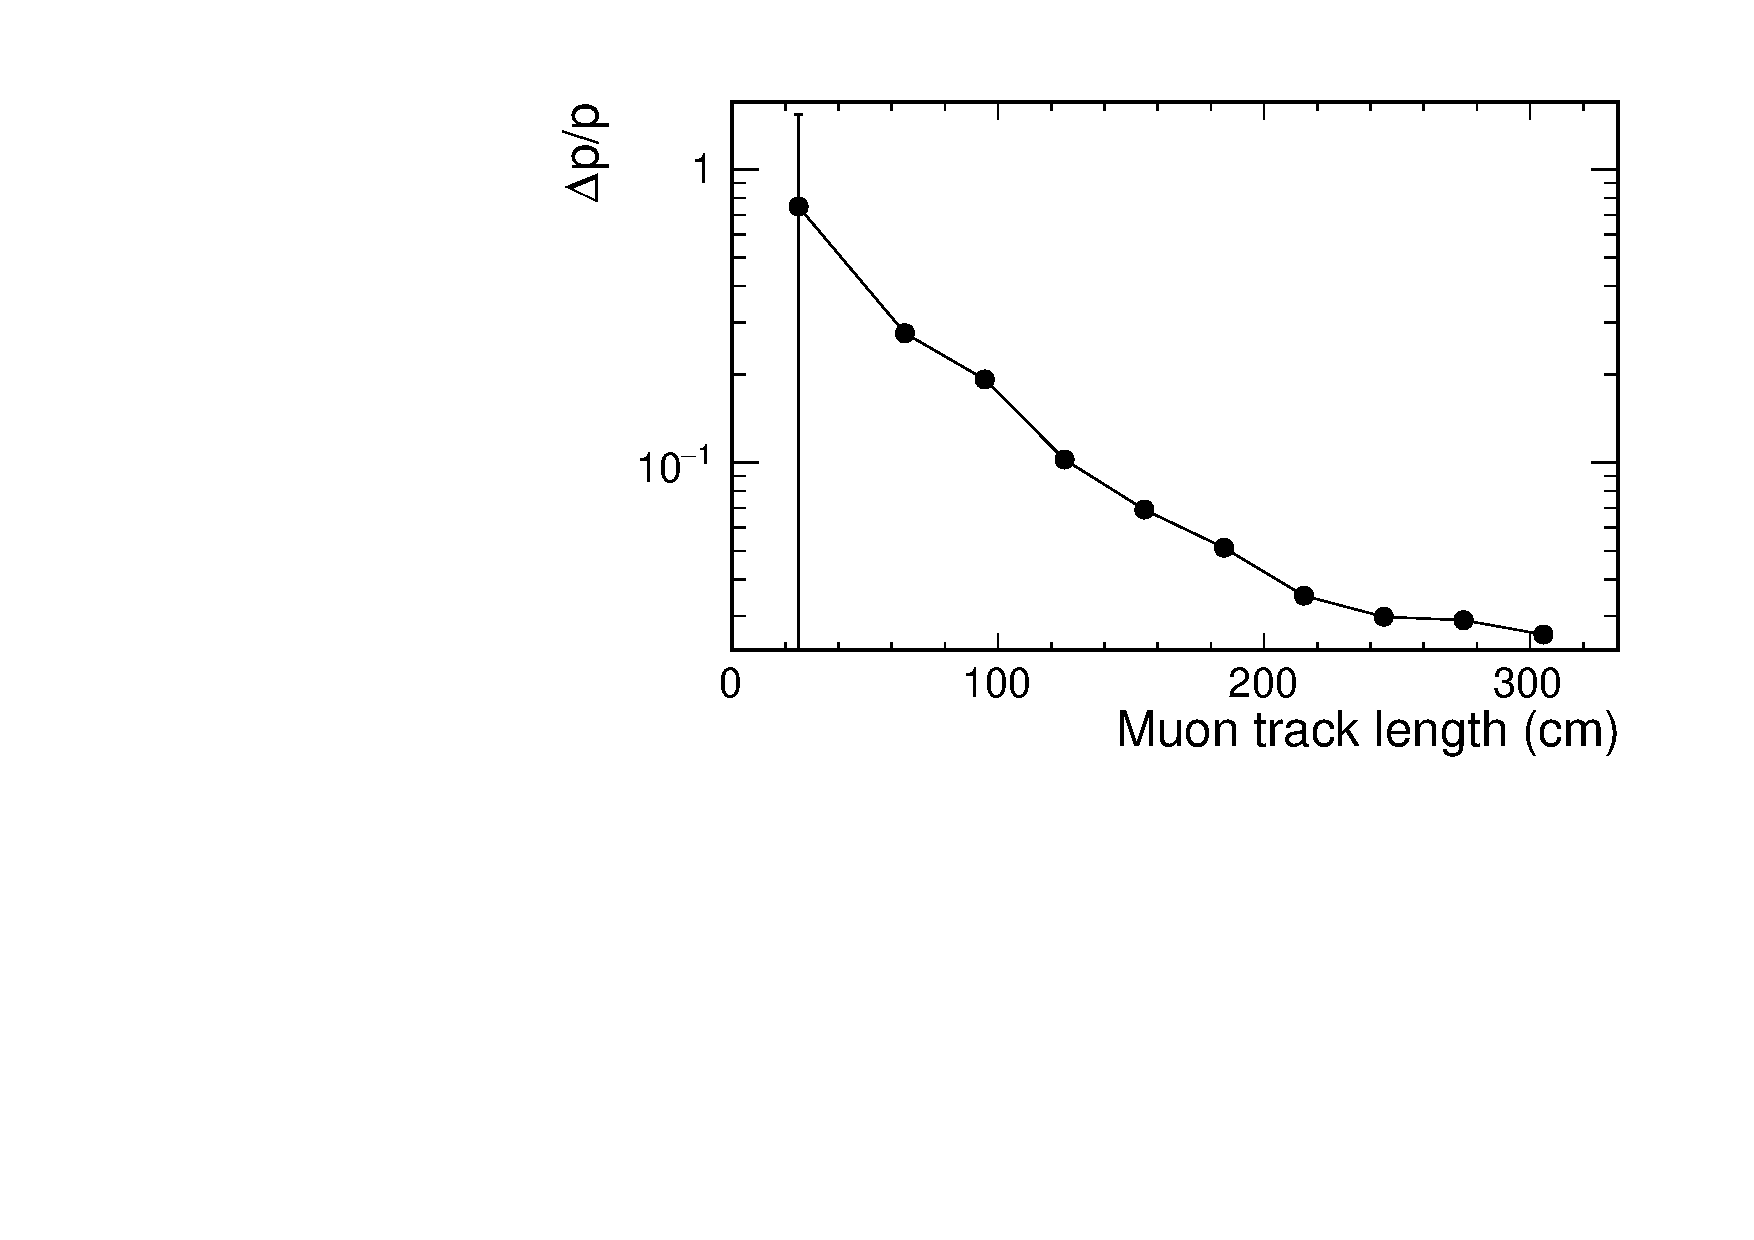
\includegraphics[width=\textwidth]{figures/ch3-DUNE/muonpoverpfunc.pdf}
         \caption{}
         \label{fig:GArTPCdpoverp}
     \end{subfigure}
        \caption[Momentum resolution performance of the ND-GAr detector.]{(Top) Momentum resolution for reconstructed muons in \texttt{GArSoft}, in a sample of $\nu_\mu$ CC events. The events were generated using the LBNF flux. The Gaussian fit to the central core of the $\Delta p/p$ distribution, containing 2/3 of events, has a width of 2.7\%. The tails are well described by a 12\% resolution. (Bottom) Momentum resolution as a function of track length \cite{DUNE:2021NDCDR}. }
        \label{fig:GARTPCdp}
\end{figure}

The resolution of a curvature momentum measurement in a TPC depends on the pad resolution as well as the multiple coulomb scattering (MS) degradation. The characteristics of the track and of the neutrino event also influence the curvature resolution. These include the particle's transverse momentum $p_T$ the track's length as well as the detector's occupancy at the time of the track formation. Given the randomized nature of particle track formation in a neutrino experiment, the distribution of the tracks length is expected to have a significant component of short tracks. For this reason fiducial cuts are imposed inside the TPC. Note that low energy particles that stop within the detector (primarily protons) would be reconstructed via their track length rather than their curvature. Within the fiducial volume ND-GAr will have a $4\pi$ acceptance. This include particles crossing the central cathode region, which is very thin (25 $\mu m$ of mylar).

An early study was done using the GArSoft software suite, on the momentum resolution for muons coming from $\nu_\mu$ CC interactions in the HpGTPC using the LBNF flux. A fiducial cut was imposed on the interaction vertexes requiring a distance of at least 50 cm from the barrel walls and 30 cm from the end-caps. The momentum resolution was calculated in terms of fractional residuals defined as:
    \begin{equation}
        \frac{\Delta p}{p_\textrm{true}} = \frac{p_\textrm{reco}-p_\textrm{true}}{p_\textrm{true}}
    \end{equation}
where $p_\textrm{true}$ is the true initial momentum of the particle while $p_\textrm{reco}$ is the reconstructed one. The distribution was fitted with a double Gaussian function defining a "core" and a tails resolution. The resolution defined by the $\sigma$ of the residual distribution is of 2.7\% for the core distribution and 12\% for the tails as shown in Fig. \ref{fig:GArTPCdp}. The single Gaussian resolution is shown as a function of the muon track length in Fig. \ref{fig:GArTPCdpoverp}.

\subsection{The electro-magnetic calorimeter}
The main role of the ECAL will be to reconstruct electrons and photons coming from neutrino interactions. The ability of detecting photons and identifying their production point makes the reconstruction of $\pi_0$ from inside the HpGTPC possible. This will be especially important in the reconstruction of $\nu_e$ events for which the missed identification of $\pi_0$ produces important systematic uncertainties. The ECAL will also be important in determining the $t_0$ for particles coming from ND-LAr and rejecting external background such as rock muons and neutrons. It will offer a time precision at the sub-nanosecond level.

The reference design of the ECAL is heavily inspired by the CALICE hadron calorimeter from the ALICE experiment \cite{CALICE:2010fpb} as well as the ECAL of the ND280 modules at T2K \cite{T2KUK:2013wkh}. It will have an octagon shape fully contained in the pressure vessel, with each octant composed by trapezoidal modules. The modules will contain alternating layers of active polystirene scintillator read out by SiPm's and absorber sheets. The active layers are segmented in tiles and strip offering an effective space resolution of the order of a few cm's.

\begin{figure}[t]
     \centering
     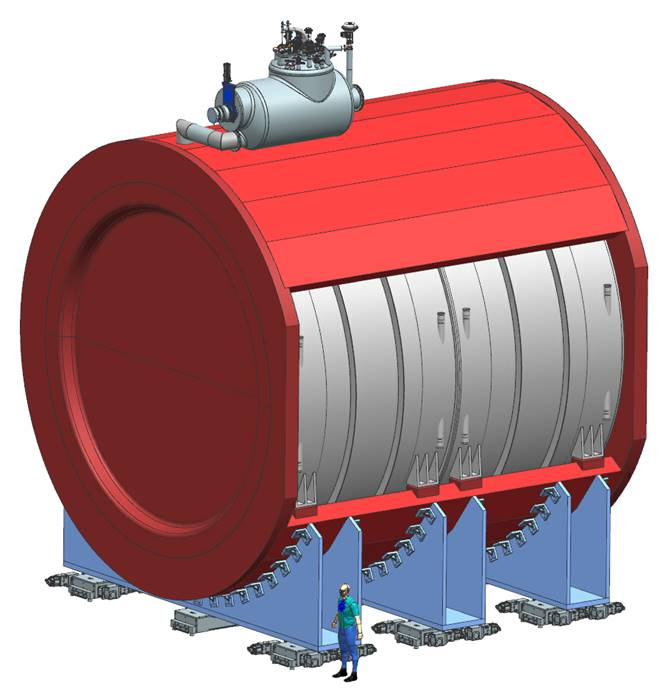
\includegraphics[width=0.6\textwidth]{figures/ch3-DUNE/Spy.jpg}
     \caption[Schematic representation of the outer layer of the SPY magnet]{Schematic representation of the outer layer of the SPY magnet, showing parts of the cryostat sytem at the top, the outer steel yoke in red, the low material budget muon window cut-out in grey and a human figure for size reference at the bottom \cite{Bersani:2023rlw}.}
        \label{fig:Spy}
\end{figure}

\subsection{The SPY magnet system}
\label{Sec:SPY}
The current integrated design for ND-GAr's solenoid, pressure vessel and yoke is named the Solenoid with Partial return Yoke (SPY) \cite{Bersani:2023rlw} and is largely based on the magnet system developed for the Multi Purpose Detector (MPD) at the NICA Collider at JINR \cite{Golovatyuk:2016zps}. The magnet system is composed of a superconducting magnet surrounded by an iron return yoke. To reduce dimensions and overall costs, the magnet and cryostat system has been designed to serve as the cylindrical component of the pressure vessel for the HpGTPC, while also providing support for the HpGTPC and the ECAL, which will be fully contained inside its volume.

The magnet coil is composed of rectangular superconducting cables bent and grouped to form six identical sub-coils with an internal diameter of 7 m, a length of 0.9 m and a thickness of 20 mm, operating at 5000A. The coils will be hosted in a cryostat reaching operating temperatures of 4.5 K to 4.7 K. The cooling elements of the cryostat will consist of pipes welded onto the outer surface of the coil formers hosting a flow of liquid helium. 

SPY's magnet will produce an overall magnetic field of 0.5 T with a field uniformity of $\pm 1\%$. These field characteristics surpass the requirements necessary to achieve the particle reconstruction performance desired by ND-GAr. These include a minimum 3\% momentum resolution for muons exiting from ND-LAr and a performance at least as good as the FD for particles produced in neutrino interactions on gas. The yoke has also been designed to reduce the amount of material between ND-LAr and ND-GAr to a minimum by removing a portion of the downstream barrel. This is important to ensure that the muons coming from ND-LAr loose as little energy as possible in un-instrumented portions of the detectors, reducing the relative uncertainties to a minimum.

SPY is completed by a carbon steel return yoke, which presents several unique characteristics. The pole faces of the yoke have been designed to offer sufficient mechanical strength to act also as the end-caps of the detector's pressure vessel. This removes the necessity for the large domed heads that would normally be required for a pressure vessel of such a diameter, shortening the overall dimensions of the system by about 4m. A schematic view of the outer components of the SPY magnet are shown in Fig. \ref{fig:Spy}.

\section{The temporary muon spectrometer}
\label{Sec:TMS}
As mentioned in Sec. \ref{Sec:DUNEfacilities}, due to budgetary restrictions, the DUNE experiment will follow a staged approach to its construction. During Phase I the muon spectrometer component of the ND complex will consist of a Temporary Muon Spectrometer (TMS) which will act as a place-holder for the ND-GAr detector, only fulfilling the minimal goals necessary for the early life of the experiment. In this section we discuss the official TMS design chosen by the collaboration (Sec. \ref{Sec:TMS-Official}), as well as an alternative design named ND-GAr-Lite (Sec. \ref{Sec: DUNE-GArLite}). While the latter design has now been abandoned by the collaboration, the studies described in Chapter \ref{ch:4-KF-NDGArLite} are centered on it, making a description of the detector necessary.

\subsection{TMS}
\label{Sec:TMS-Official}
\begin{figure}[t]
     \centering
     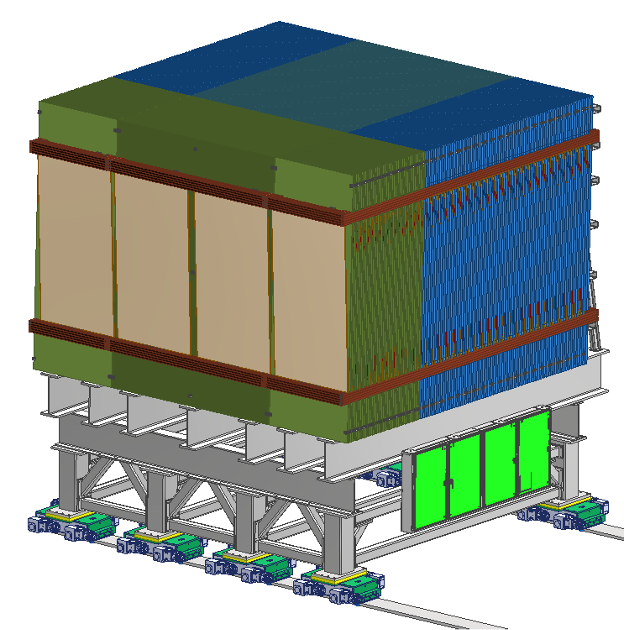
\includegraphics[width=0.6\textwidth]{figures/ch3-DUNE/TMS.png}
     \caption[Schematic view of the temporary muon spectrometer's current official design.]{Schematic view of the temporary muon spectrometer's current official design \cite{Battisti:2022ND}.}
        \label{fig:TMS}
\end{figure}
The temporary muon spectrometer (TMS) is a magnetized steel range stack detector which is set to become operative during DUNE Phase I. Its main role will be to measure the momentum and charge of muons exiting ND-LAr. This will increase the acceptance of ND-LAr making the performance of the two combined detectors comparable to that of the FD \cite{DUNE:2022aul}.

Both the Argon target and the technology of ND-LAr are essential to predict the rate and spectrum of neutrino-argon interactions expected at the FD and achieve the level of control over the systematics necessary for the Phase I physics goals. The inclusion of a magnetized muon catcher to ND-LAr is important to improve the muon momentum reconstruction performance in the key energy range between 0.5 and 5 GeV reaching a resolution of the order of $\delta p / p \sim 5\%$. The sign selection, which is not available using ND-LAr alone, is crucial in the $\delta_\textrm{CP}$ measurement. This is especially true in reverse horn current where the beam will experience a large contamination of neutrino interactions comparable to the desired anti-neutrino interactions. In measuring $\Bar{\nu}_e$ appearance, the sample of $\nu_e$ interactions needs to be carefully accounted for.

TMS consists of 100 alternating layers of magnetized steel absorber and plastic scintillator. A schematic representation of the detector is shown in Fig. \ref{fig:TMS} . Each scintillator layer consists of four panels divided into 48 strips, all 300 cm long and 3.5 cm wide. The strips in each layer are tilted in an alternating pattern by $\pm 3^\circ$ with respect to the vertical direction, providing U and V views. Each layer of steel will be divided into three columns, each magnetized by two electrified coils. The coils which surround the central block produce a magnetic field which faces downwards, while the two later blocks have a magnetic field pointing  in the opposite direction. The thickness of the steel plates is of 15 mm for the first 40 layers upstream and of 40 mm in all the others. The thickness of the steel layers was chosen in order to optimize the particles' energy deposition.

In TMS the muon momentum will be measured by range, while the charge sign will be determined based on the curvature of the particle trajectory. The scintillator layers are instrumented with ADC's and can provide calorimetric information as well as position measurements. This information can be used in many ways: the Bragg peak can be used to identify stopping muons more effectively; muons experiencing very high energy loss via bremmstrahlung can be selected and more effectively reconstructed; the stopping point can be more effectively found by studying the evolution of $1/\beta^2$ along the track. Calorimetric measurements of muon energy can also be made but they are not expected to be competitive with the range measurements. 

The capabilities of TMS will be sufficient to reach the physics goals of the DUNE collaboration during Phase I, where the uncertainties will be dominated by the lack of statistics. This won't be true for Phase II where the impact of the systematics will be much larger. This is why TMS will be substituted by a more capable Near Detector (MCND) module, the leading design currently corresponding to ND-GAr. 

\subsection{ND-GAr-Lite}
\label{Sec: DUNE-GArLite}

ND-GAr-Lite was an alternative Phase I muon spectrometer design for the ND which would have become possible in the case that early funds for the construction of the SPY magnet had become available \cite{ND-GAR-LiteCDR} (see Fig. \ref{fig:Lite} for a schematic representation of the design). The detector would have included all the components of the SPY system while the central volume of the magnet would have been instrumented with a minimal amount of scintillator tracking planes. The advantage of this approach was to provide a natural staging to the construction of ND-GAr, reducing overall cost and wastes compared to the nominal TMS design, which is set to be fully removed from the ND in the transition between Phase I and II. The ND-GAr-Lite design was eventually abandoned by the collaboration as it became clear that the funds necessary to build the SPY magnet were not going to be available for Phase I. 

Two plans were originally envisioned for the transition between ND-GAr and ND-GAr-Lite. The first approach was the most straightforward and consisted in building the ECAL and HpGTPC above ground and lowering them in the ND chamber at the same time. They would have been then mounted inside the already functioning spy magnet and enclosed inside the pressure vessel. The estimated shut-down for such a scenario would have been of the order of 8 months, similar to the 6 months estimated for TMS. The second plan consisted in a staged approach where the ECAL would have been inserted first, while keeping the tracking planes in place. The HpGTPC would have been inserted soon after completing the design. This staged approach had the potential to reduce beam shut-down to a minimum but was never fully studied.

\begin{figure}[t]
     \centering
     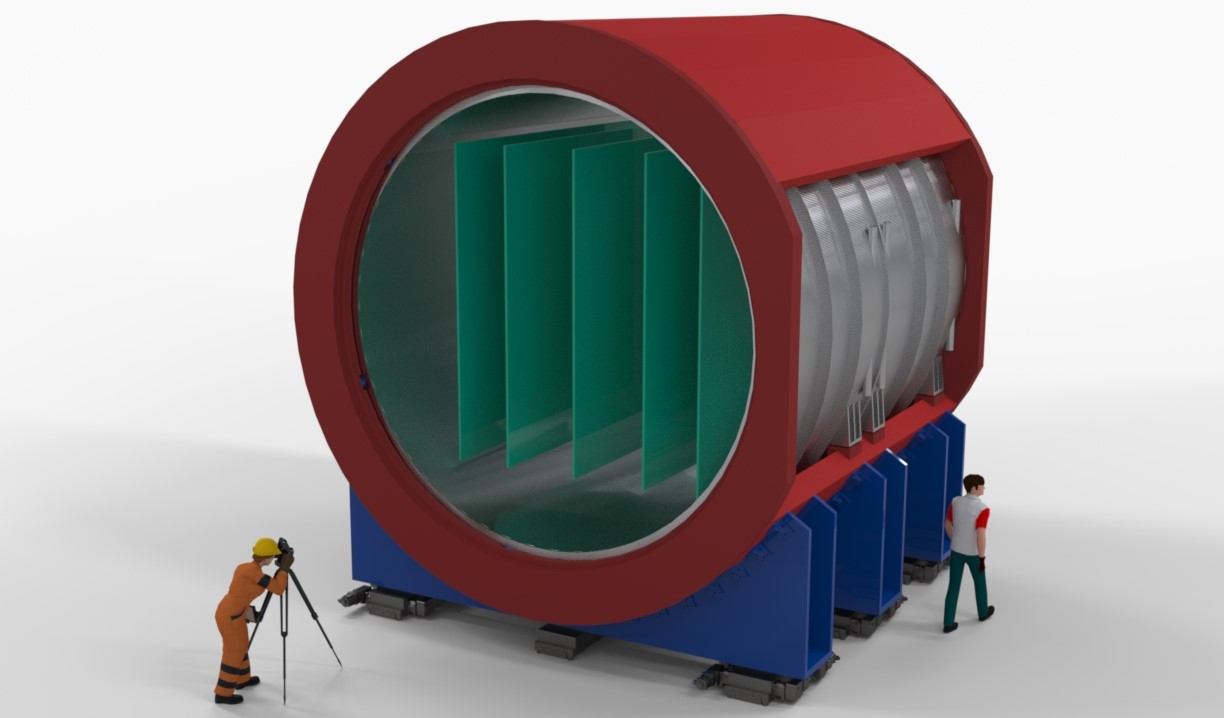
\includegraphics[width=0.8\textwidth]{figures/ch3-DUNE/MPD_Magnet_w_Tracker_Planes.jpg}
     \caption[Rendering of the ND-GAr-Lite TMS design]{Rendering of the ND-GAr-Lite TMS design. The return yoke end caps are removed to show the inner region \cite{ND-GAR-LiteCDR}.}
        \label{fig:Lite}
\end{figure}

The nominal design for ND-GAr-Lite’s tracker consisted of a series of rectangular tracking stations, all roughly 5.8m tall and 5.1m tall, positioned perpendicularly to the beam direction. Each plane would have included a x-plane and a y-plane composed of triangularly shaped scintillator bars, approximately 4cm wide and 2 cm tall. Each bar would have been equipped with a detector module called quad-counter, which would have included a motherboard reading out 4 SiPMs which could detect the light from 4 wavelength-shifting fibers. An additional muon tagger plane to be placed between ND-LAr and ND-GAr-Lite was also considered by the collaboration. This muon-tagging system would not have been removed in the transition between Phase I and II and would have been especially useful to ND-GAr for $\mu/\pi$ separation. A muon-tagging system is still being considered by the collaboration but no mature design exists.  

In order to form a track, ND-GAr-Lite required at least three hits in three unique planes. The nominal tracker design included 5 planes, placed symmetrically about the center of the internal cylinder of the detector. This configuration was eventually substituted by a new design which used 6 unequal planes, mostly placed in the upstream half of the ND-GAr cryostat. The nominal design had a tracking momentum threshold for muons exiting ND-LAr of 1 GeV/c and an angular acceptance of $\sim$ 20 deg. The new arrangement extended the tracking capability to cover nearly all of the muon kinematic phase space, improved the overall tracking efficiency, and lowered the threshold to track muons with initial momenta as low as 700 MeV/c. Regardless of the planes disposition, the relative momentum resolution for ND-LAr muons was estimated to be between 2\% and 4\% over a wide range of momenta. These results satisfied the $\leq 4\%$ ND requirements for a Phase I muon spectrometer.  

\section{Dune's scientific program}
\label{Sec:DUNEscientific}
The primary scientific goal of the DUNE experiment consists in performing a comprehensive set of neutrino oscillation measurements using the $\nu_\mu$ and $\Bar{\nu}_\mu$ beams coming from LBNF at Fermilab. Particularly central amongst these measurements are the determination of the charge parity phase $\delta_\text{CP}$, the neutrino mass ordering (i.e. the sign of $\Delta m_{31}^2$) and the octant in which the mixing angle $\theta_{23}$ lies. Other key goals of the experiment include the search for proton decay in several decay modes and the detection and measurement of $\nu_e$'s from a core-collapse supernova within the Milky Way, were that to occur during the lifetime of the experiment. DUNE will also pursue a series of secondary research topics such as beyond the Standard Model (BSM) searches and measurements of neutrino oscillations using atmospheric neutrinos. All these topics will be introduced and discussed in this section. The DUNE ND will offer its own complementary physics program, which will be discussed separately in Sec. \ref{Sec:NDScientific}.


\subsection{Neutrino oscillation measurements}
The central aim of DUNE is to test the three-flavour neutrino oscillation paradigm at an unprecedented level of precision. It will do this by performing neutrino oscillation parameter measurements which will allow to shed light on key questions in the field. The neutrino mass ordering remains undetermined, with current measurement only marginally preferring the normal hierarchy hypothesis.  The value of $\delta_\textrm{CP}$ is poorly constrained with all possible values in the range between $\pi$ and $2\pi$ being consistent with data. Finally the value of $\theta_{23}$ is known to be close to the maximal mixing value $\pi/4$ but its octant is still unresolved. DUNE aims to provide answers to all these open questions.

In long-baseline experiments such as DUNE that have access to horn-focused beams producing either $\nu_\mu$ or $\bar{\nu}_\mu$ dominant fluxes, the oscillation parameters can be studied either through disappearance or appearance measurements. An appearance measurement refers to the detection of a neutrino flavor that was not present in the initial neutrino beam, while a disappearance measurement involves detecting a reduction in the number of neutrinos of a specific flavor as they travel over a certain distance, compared to what is expected if no oscillation occurred. Due to the almost maximal value of $\theta_{23}$ the $\nu_\mu\rightarrow\nu_\tau$ is the dominant flavour oscillation. Due to the fact that the oscillation maxima occur at energies below the threshold for $\tau$-lepton production in $\nu_\tau$ CC interactions, these types of oscillations can only be studied through disappearance measurements. On the other hand the sub-dominant channel $\nu_\mu\rightarrow\nu_e$ allows for the detailed study of many oscillation properties through the measurement of the $\nu_e$ and $\bar{\nu}_e$ spectra.

If we assume a constant matter density the oscillation probability $\nu_\mu\rightarrow\nu_e$ can be written as:
\begin{equation} \label{eq1}
    \begin{split}
        P(\nu_\mu\rightarrow\nu_e) & = \sin^2\theta_{23} \sin^22\theta_{13} \frac{\sin^22(\Delta_{31}-aL)}{(\Delta_{31}-aL)^2}\Delta_{31}^2\\
         &  +\sin2\theta_{23} \sin2\theta_{13} \sin2\theta_{12} \frac{\sin^22(\Delta_{31}-aL)}{(\Delta_{31}-aL)}\Delta_{31}\\
         & \times\frac{\sin(aL)}{(aL)}\Delta_{21} \cos(\Delta_{31}+\delta_\textrm{CP})\\
         & +\cos^2\theta_{23} \sin^22\theta_{12} \frac{\sin(aL)}{(aL)}\Delta_{21} \Delta_{21}^2
    \end{split}
\end{equation}
where $\Delta_{ij}=\Delta m_{ij}^2L/4E_\nu$ is the phase difference, $a = G_FN_e\sqrt{2}$ is the matter effect coefficient, $G_F$ is the Fermi constant, $N_e$ is the number density of electrons in the Earth, $L$ is the baseline in km, and $E_\nu$ is the neutrino energy in GeV. In the equation above, both $\delta_\textrm{CP}$ and $a$ switch signs going from the $\nu_\mu\rightarrow\nu_e$ to the $\bar{\nu}_\mu\rightarrow\Bar{\nu}_e$ channel which implies that a neutrino-antineutrino asymmetry is introduced both by CP violation ($\delta_\textrm{CP}$) and the matter effect ($a$). As explained in Sec. \ref{Sec:MSW} the matter effect asymmetry simply arises from the presence of electrons in the Earth's matter, with which $\nu_e$'s have a high probability to interact and $\bar{\nu}_e$ do not. In the few GeV range the interaction probability of $\nu_e$'s and thus the impact of matter effect increase with the amount of matter traversed by the neutrino. Experiments with longer baselines are thus more sensitive to matter effects and consequently to the mass ordering. DUNE, with its 1300km baseline, will be able to resolve the degeneracy between the MSW and CP-violating asymmetry and determine both the neutrino mass ordering and the value of $\delta_\text{CP}$ at $5\sigma$ for more than 50\% of its possible true values \cite{Diwan:2004bt}.

The measurement of $\delta_\text{CP}$ in DUNE also benefits from the use of a wide-band neutrino beam. In Fig. \ref{fig:energy_nu} we show the $P(\nu_\mu\rightarrow\nu_e)$ as a function of neutrino energy at a 1300 Km baseline for three maximal values of $\delta_\text{CP}=-\frac{\pi}{2},0,\frac{\pi}{2}$. The various oscillation nodes are clearly visible, with the main one being peaked at 2.4 GeV, where DUNE's neutrino flux will also be peaked. The value of $\delta_\text{CP}$ impacts both the amplitude and the phase of the oscillation nodes: for this reason being capable of measuring the rate of $\nu_e$ appearance as a function of the neutrino spectrum is highly desirable. In particular the impact of $\delta_\text{CP}$ on the amplitude of the oscillation probability peaks is higher at nodes below neutrino energies of 1.5 GeV, making the ability of DUNE of measuring $\nu_e$ appearance down to at least 500 MeV highly impactful.

While the determination of the neutrino mass hierarchy and the discovery of CP-violation in the leptonic sector will be the main goals of DUNE's oscillation program, the measurements of all the other parameters regulating the oscillation probability will also be a key focus. Particular importance will be given to the measurement of the the mixing angles $\theta_{13}$ and $\theta_{23}$. The $\theta_{13}$  mixing angle has been accurately measured in reactor experiments, which will provide constraint to the DUNE oscillation analysis in the early stages of the experiment. However, to reach the desired levels of systematics constraint, DUNE will have to perform a measurement of $\theta_{13}$ which is independent from and competitive with the reactor results. The measurement in DUNE will be done using a $\nu_e$ and $\bar{\nu}_e$ appearance channel, whereas in reactor experiments it is performed through $\bar{\nu}_e$ disappearance.

\begin{figure}[t]
     \centering
     \begin{subfigure}[b]{0.48\textwidth}
         \centering
         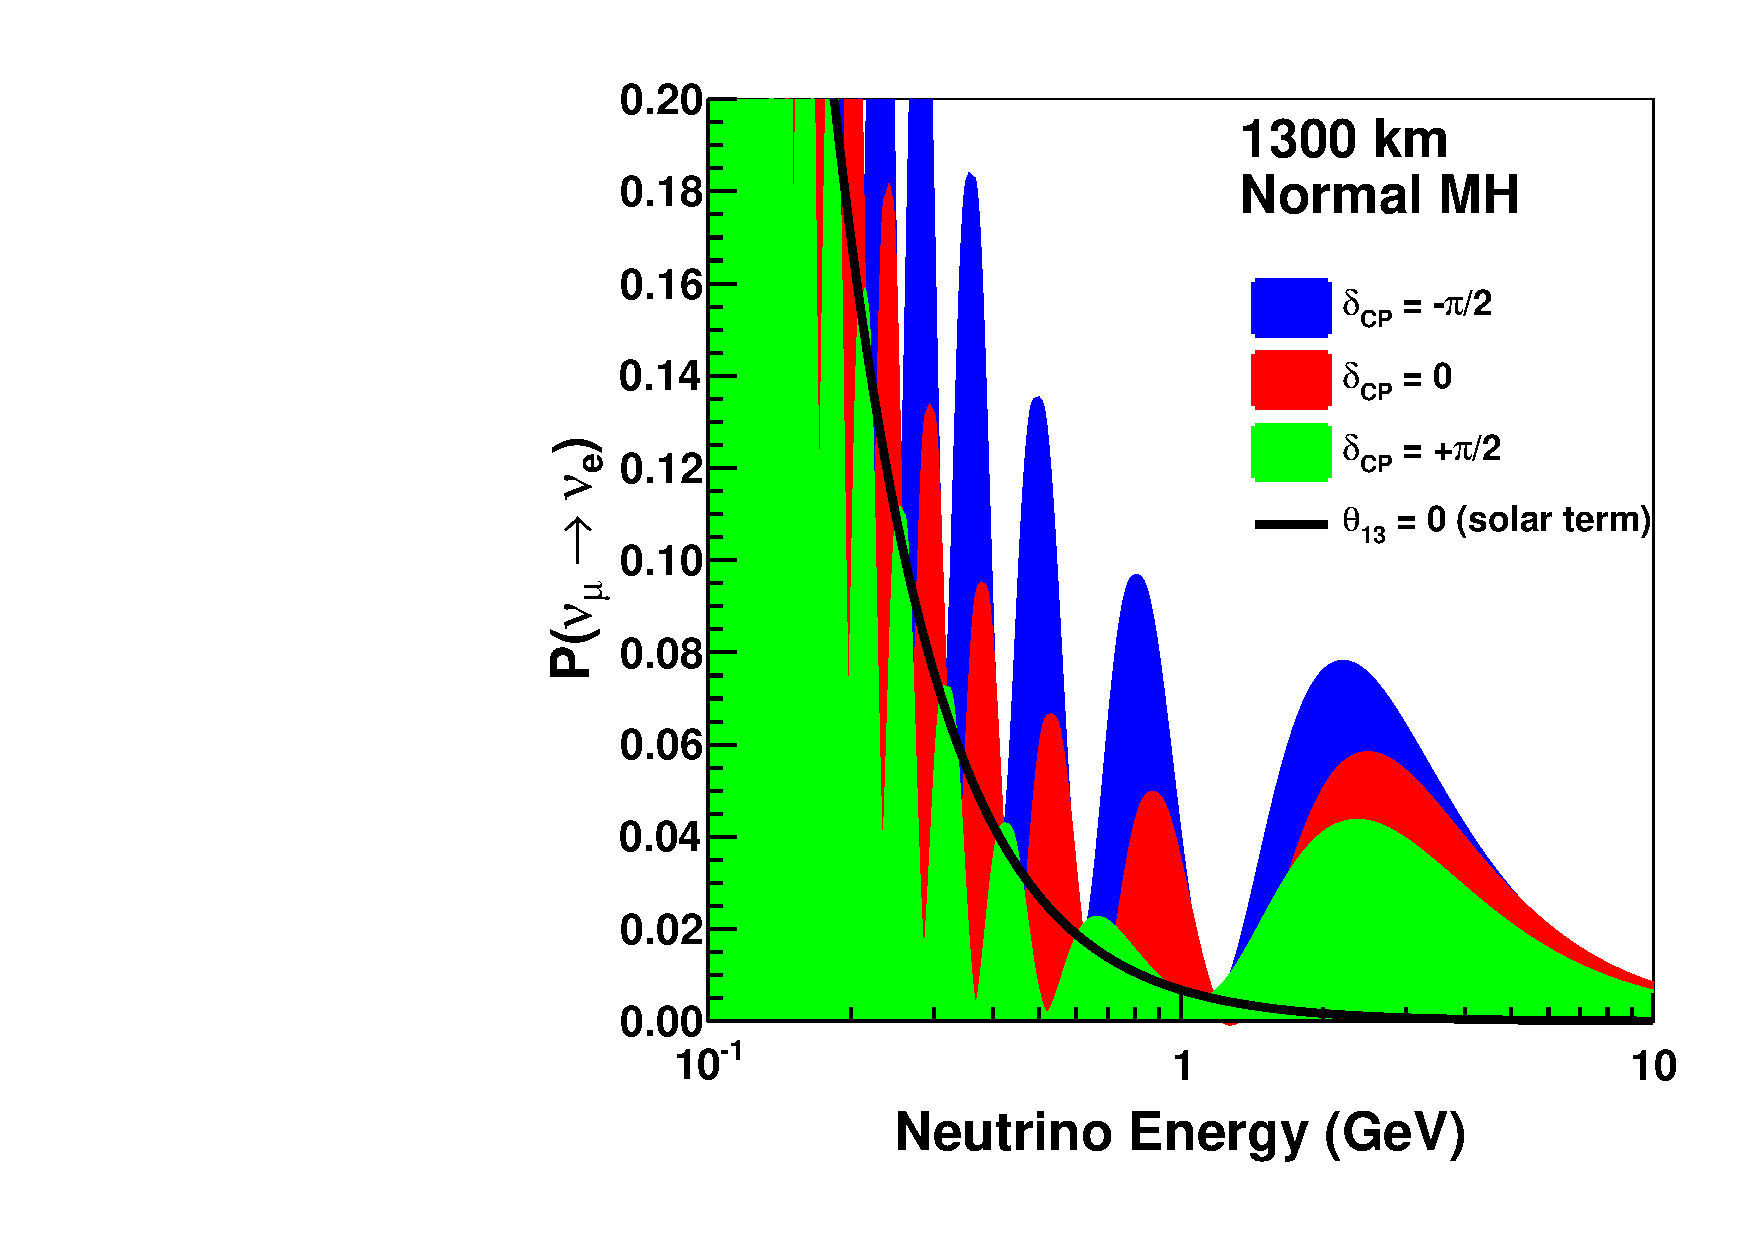
\includegraphics[width=\textwidth]{figures/ch3-DUNE/energy_nu_no.pdf}
         \caption{}
         \label{fig:energy_nu_no}
     \end{subfigure}
     \hfill
     \begin{subfigure}[b]{0.48\textwidth}
         \centering
         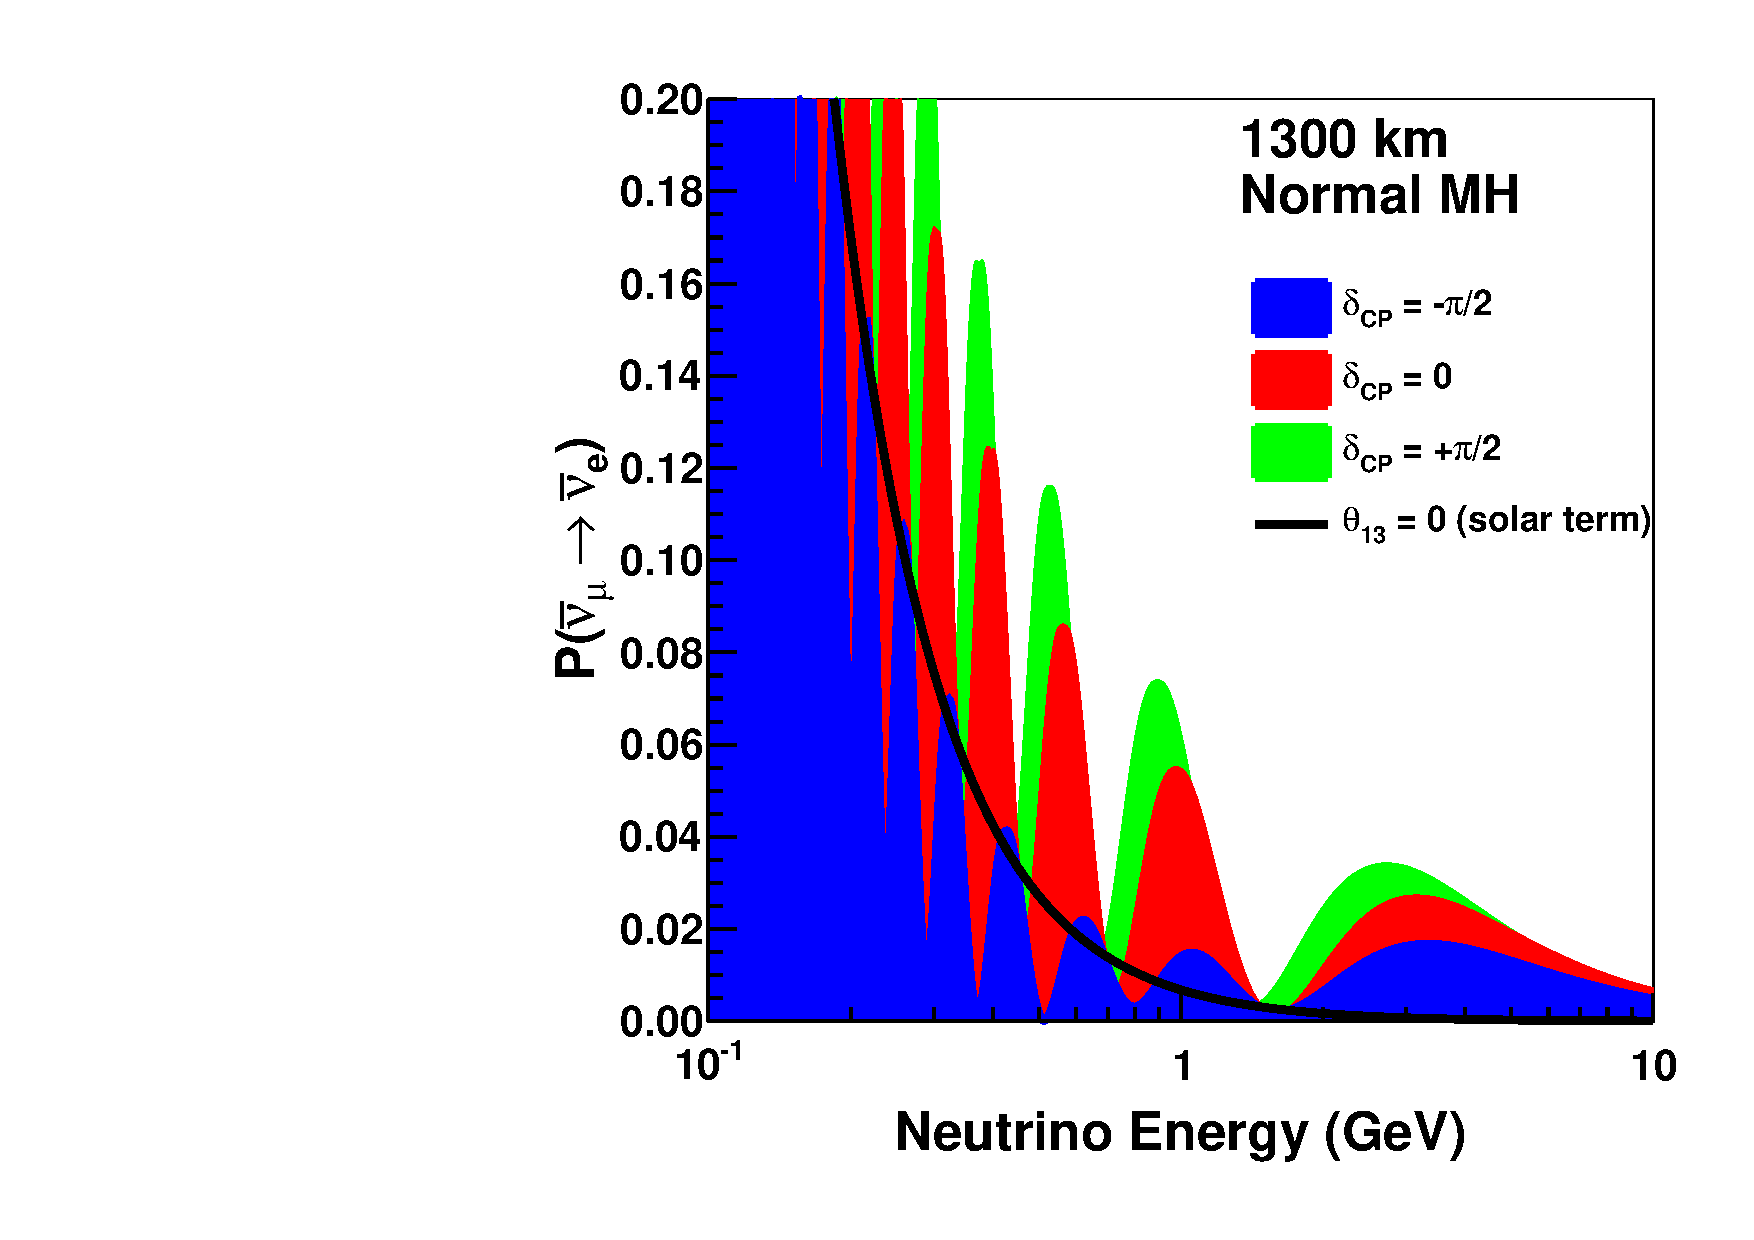
\includegraphics[width=\textwidth]{figures/ch3-DUNE/energy_anu_no.pdf}
         \caption{}
         \label{fig:energy_anu_no}
     \end{subfigure}
        \caption[Appearance probability as a function of neutrino energy.]{The appearance probability at a baseline of 1300 km, as a function of neutrino energy, for $\delta_\text{CP}$ (blue), 0 (red), and $\pi/2$ (green), for neutrinos (left) and antineutrinos (right), for normal ordering. The black line indicates the oscillation probability if $\sigma_{13}$ were equal to zero. Note that DUNE will be built at a baseline of 1300 Km \cite{DUNE:2020TDR1}. }
        \label{fig:energy_nu}
\end{figure}


The measurement of $\sin^2\theta_{23}$ in DUNE will help disambiguate its value, potentially pointing to a previously unknown symmetry between the $\nu_2$ and $\nu_3$ mass eigen-states.  Current world measurements are ambiguous on whether the values of $\theta_\text{23}$ lies in the lower octant ($<45^\circ$) or the higher octant ($>45^\circ$) and allow for the maximal value $\sin^2\theta_{23}=0.5$ \cite{Esteban:2018azc}. This would implicate that the $\nu_\tau$ flavor eigen-state receives equal contributions from the mass eigen-states $\nu_2$ and $\nu_3$, which would point towards a previously unknown symmetry. 

Overall obtaining measurements of all the oscillation parameters within a single wide-band oscillation experiment has great value, because it provides a clear analysis of the neutrino oscillation pattern allowing for a detailed test of the three-flavor neutrino model. Additionally, precise measurements of the PMNS mixing values, allow for comparison with mixing patterns in other areas of the standard model such as quarks. The question of why the quark mixing angles are smaller than the lepton mixing angles remains unanswered and constitutes an important part of the flavor pattern question \cite{King:2014nza}. 


\subsection{Nucleon decay}
\label{Sec:ProtonDecay}
Many BSM theories propose the unification of the strong, electromagnetic and weak interactions. These grand unified theories (GUT's) extend the standard model introducing a unified gauge symmetry at very high energies ($>10^{15}$ GeV) \cite{deBoer:1994dg}. One of the experimentally verifiable predictions that GUT's have in common is nucleon decay \cite{Langacker:1980js}. The dominant modes for proton decays predicted by GUT's are $p\rightarrow K^+ + \bar{\nu}$ and $p\rightarrow K^+ +\pi^0$. The first and second mode are dominant in supersymmetric and non-supersymmetric GUT's respectively. While no evidence of supersymmetry has been found at the electroweak scale, despite extensive efforts at the large hadron collider (LHC), the main appeal of GUT's, which consists in gauge-coupling unification remains intact. 

Many experiments have performed searches of nucleon decay, imposing lifetime limits which already constrain the viability of several GUT models. Currently the best limits on most nucleon decay modes are set by the Super Kamiokande experiment, which features the largest mass and exposure time (more than 30 years) of any detector to date \cite{Super-Kamiokande:2014otb, Super-Kamiokande:2016exg, Super-Kamiokande:2017gev}. Extending the lifetime limits will require detectors to feature long exposure times combined with either large sensitive masses or improved detection efficiency or background rejection. The FD LArTPC's feature all these characteristics. Their excellent imaging, calorimetric and particle identification capabilities, combined with their large liquid Argon mass, make them ideal detectors for a nucleon decay search. The LArTPC technology is particularly well suited for the $p\rightarrow K^+ +\bar{\nu}$ or any decay mode that involves charged kaons, because it allows to observe the entire decay chain. In a water Cherenkov detector such as Super Kamiokande the kaons emerging from these decay modes are usually below threshold, but in a LArTPC they can be identified both by their distinctive $dE/dx$ as well as their decay. Therefore, this mode can be tagged in a LArTPC by looking for single kaons within a suitable energy range with their point of origin lying within the fiducial volume followed by its decay products. The background induced by cosmic ray muons can be contained imposing fiducial volume cuts and stringent kaon identification requirements. The dominant background is thus produced by atmospheric neutrino interactions.

The DUNE FD will not limit its search to a single mode or a few dominant channels, but it will feature a broad program covering many decays. These efforts are made all the more interesting by the fact that during DUNE's lifetime, two other large detectors, Hyper-Kamiokande \cite{Hyper-Kamiokande:2018ofw} and JUNO \cite{JUNO:2015sjr} are set to perform searches for nucleon decays. If any of the experiments were to observe a signal, having confirmation from other experiments using drastically different detector technologies and thus different backgrounds would be very powerful.

\subsection{Atmospheric Neutrinos}
\label{Sec:AtmosphericNeutrinos}

Atmospheric neutrinos offer a complementary sample which includes all neutrino and anti-neutrino flavours and a wide range of $L/E$. This will allow for a measurement of all oscillation parameters which is independent from the one performed with the neutrino beam. Furthermore, the atmospheric sample will be available at all times, even before the Near-detector or the LBNF neutrino beam become operative, offering an ideal training ground for the development of reconstruction software, analysis methodologies, and calibrations at the FD.

The FD's, due to their large mass and overburden, which protects them from the atmospheric muon sample, are well equipped to study the atmospheric neutrino sample. Additionally atmospheric neutrinos produce event topologies which are highly overlapping with those produced by neutrinos from the beam. The only additional requirements that are needed to make the study of atmospheric neutrinos possible are a self trigger and  a more stringent demand on the neutrino direction reconstruction. The LArTPC technology is well equipped to accommodate both, thanks to its scintillation fast timing properties and its photographic reconstruction capabilities.

The atmospheric sample is especially suited to determine the neutrino mass ordering. This is due to the fact that the atmospheric neutrinos travel through the entire Earth before reaching the detectors, and are thus much more impacted by the MSW matter effect. This makes the determination of the mass ordering highly independent from the measurement of $\delta_\text{CP}$. Additionally, the sensitivity is proportional to the square root of the exposure \cite{DUNE:2020TDR1, Ternes:2019sak} , indicating that the measurement is not systematics-limited. This is in stark contrast with the mass ordering determination that can be achieved with the beam measurements for which the control of the systematic uncertainties is the main limiting factor. The sensitivity to mass ordering using the atmospheric sample can be greatly improved if separation between neutrinos and anti-neutrinos can be achieved. This is not straight-forward in DUNE's FD's, since they lack magnetization. However thanks to their high resolution imaging capabilities, particle/anti-particle statistical discrimination can be achieved through topological tagging. 

Many other important measurements can be made using atmospheric neutrinos at the DUNE FD's. Studies have indicated that it could be possible to use a sample of sub-GeV atmospheric neutrinos to exclude some regions of $\delta_\text{CP}$ independently from the beam measurements \cite{Kelly:2019itm}. Additionally atmospheric neutrinos can act as a probe for many BSM scenarios, potentially allowing DUNE to place competitive limits on Lorentz and charge, parity, and time reversal symmetry (CPT) violation (similarly to what has been done by the IceCube \cite{IceCube:2010fyu,IceCube:2017qyp} and Super-Kamiokande \cite{Super-Kamiokande:2014exs} collaborations) non-standard interactions \cite{Chatterjee:2014gxa} and sterile neutrinos \cite{Super-Kamiokande:2014ndf}.
\subsection{Supernova neutrinos}
\label{sec:SupernovaNeutrinos}

A core-collapse supernova is an end of life event which occurs when all the nuclear fuel present in a massive star is consumed. In the late stages of such a star's life, as an effect of nucleo-genesis and nuclear burning, its core assumes a concentric structure, with iron at the center and progressively lighter elements moving outwards. Once temperatures of $T\sim10^{10}$ K are reached, the iron core loses energy by neutrino emission through pair annihilation and plasmon decay. Simultaneously, the Fe nuclei are too heavy to be further burned for energy production, and thus the core contracts and heats up while also increasing its mass through additional nucleo-genesis. Once the critical Chandrasekhar mass of 1.4 solar masses is reached, the pressure imposed by the external layers of the star can no longer be balanced and the star almost immediately collapses. The central core bounces and produces an initial shock wave. At the same time the iron core reaches nuclear levels of density storing most of the gravitational energy in the form of a degenerate Fermi sea of electrons and electron neutrinos. Eventually the trapped energy is released mostly in the form of $\sim 10^{58}$ $\nu_e$'s with energies of $\sim10 \ \text{MeV}$. The central object then settles to a neutron star or a black hole and the remaining energy is absorbed by beta reactions behind the shock wave that blasts away the rest of the star, resulting in the supernova explosion.

As the majority of the energy in a supernova core-collapse is released through the expulsion of $\nu_e$'s, neutrinos represent an essential probe in the study of these phenomena. This was proven when electron antineutrinos from the SN 1987a core collapse were detected via Cherenkov and scintillation detectors \cite{Bionta:1987qt, Kamiokande-II:1987idp}. While the amount of statics gathered during this event was sparse, the observations provided a qualitative validation of the basic physical structure of the supernova collapse phenomenon. The current generation of detectors will make a high statistics observation of a nearby supernova possible, with sensitivity to different flavour components of the flux. This is particularly important because the different phases of the core-collapse neutrino production are expected to produce distinct neutrino flavour and energy spectra, the evolution of which can be studied to shed light on the supernova process and the nature of neutrinos themselves. 


The DUNE FD's will be sensitive to supernova neutrinos with energies down to 5 MeV to a few 10's of MeV's. The FD's LArTPC's are expected to be particularly sensitive to the $\nu_e$ component of the supernova burst through the CC absorption channel $\nu_e+^{40}Ar \rightarrow e^-+^{40}K^*$, where the $^{40}K^*$ represents a potassium nucleus in an excited state. The exiting electron combined with the de-excitation products of the $^{40}K^*$ nucleus provide a particularly clean signature which is not available to other neutrino detector technologies. Other electron flavor channels available to the FD include $\Bar{\nu}_e$ CC interactions and elastic electron scattering. Additionally it is possible that other core-collapse neutrino flavours will be accessible through neutral current interactions such as $\nu+^{40}Ar \rightarrow \nu+^{40}Ar^*$ where the products of the de-excitation of the Argon nucleus can be used for tagging. This possibility is however yet to be investigated. 

 


\subsection{Beyond the standard model physics}
\label{sec:BSM}

The combination of the high intensity wide-band LBNF neutrino beam with a highly capable ND and a massive LArTPC FD make DUNE an ideal experiment for many searches of new physics. In this section we summarize some of the key searches that have already been proposed and in some cases investigated by the DUNE collaboration.

An important field of study in neutrino physics consists in exploring the possibility of extending the standard three-flavor paradigm. Experimental results exist which are in tension with the SM and can be interpreted as mixing between the currently known neutrino flavours and one or more sterile states \cite{Gariazzo:2017fdh, Dentler:2018sju}. These results have produced a wide field of  searches for sterile neutrinos through many different experiments and methodologies. DUNE will be able to search for a wide range of sterile neutrino masses by looking for missing NC and CC interactions both at the FD's long baseline as well as the ND. Additionally, anomalies pointing towards the expansion of the three flavour paradigm in the standard model could be found by measuring deviations from the unitarity of the PMNS matrix, something that can be done by DUNE by measuring the oscillation parameters at unprecedented levels of precision. These deviations would be particularly sizeable if the masses of the extra states are relatively small. 

If the DUNE data is consistent with the 3-flavor hypothesis, non-standard interactions could still effect the propagation of neutrinos through the Earth \cite{Farzan:2017xzy}. Thanks to its very long baseline and wide-band beam, DUNE could be sensitive to these anomalies if the parameters that regulate the new physics are large enough. One of the ways in which DUNE will investigate the existence of non-standard interactions, is through the measurement of  neutrino-induced di-lepton production in the Coulomb field of a heavy nucleus, also known as neutrino trident interactions \cite{Altmannshofer:2019zhy}. These channel, while extremely rare, is a particularly sensitive probe into the existence of new gauge symmetries beyond the SM. Thanks to the high intensity of the LBNF beam a relatively large amount of these interactions are expected at the ND ($\sim 100$ trident interactions per year), making DUNE capable of measuring deviations from the SM rates and test the presence of new gauge symmetries.

The characteristics of the DUNE experiment also make it particularly well positioned to test various models of light dark matter (LDM). The existence of dark matter is very strongly supported by many cosmological and astrophysical observations, however no direct detection of weakly interactive massive particles has been done so far \cite{Planck:2018vyg}. It has been proposed that if the DM is much lighter than the electroweak scale, then DM candidates could exist that interact with regular matter through a \enquote{vector portal} mediator could be well justified \cite{Battaglieri:2017aum}. It has been shown that high flux neutrino beam experiments such as DUNE could be sensitive to such DM candidates, whereas collider experiments such as the LHC are not. Another important category of dark matter that could be accessible to DUNE though its large LArTPC FD's, is the so-called boosted dark matter (BSM) \cite{Agashe:2014yua}. Many models exist that contain both a heavy and light DM component, in which the lighter one can be produced from the annihilation of the heavier one in environments with high DM concentrations such as the Sun or galactic centers. Due to the large mass difference between the two DM components, the lighter one is produced with a relativistic boost, making it energetic enough to be detected by the DUNE FD's in a wide range of parameter space.

\section{Near detector physics}
\label{Sec:NDScientific}

The design of DUNE's near detector is completely informed by the necessities of the experiment's oscillation measurement program. The ND will serve as the experiment's control: it will establish the no oscillation hypothesis under the three neutrino paradigm, measure and monitor the beam, constrain systematic uncertainties and provide essential input to interaction models.

The oscillation measurement directly depends on the neutrino spectra that are established at the ND. Only using these measurements it is possible to predict the un-oscillated neutrino energy spectra at the FD and obtain a measurement of the oscillation parameters through a fit. The picture is complicated by the fact that the reconstructed neutrino spectrum at the FD is an unresolved convolution of cross section, flux, and energy response. The ND must independently constrain all of these components and provide information which can improve the precision of the models. For this reason the ND must significantly outperform the FD: multiple methods to determine neutrino fluxes with differing dependencies on the cross-sections need to be available, and the cross sections need to be measured to a high degree of precision. Additionally the ND needs to be capable of measuring events in a similar way to the FD,  mitigate environmental differences and confidently predict the FD event rates, while also operating in a much higher rate environment. The ND is designed to achieve all these scientific goals while also providing its own independent program of BSM and SM physics.

\subsection{Flux measurements}
\label{Sec:Flux}

In order to understand the importance of the ND in achieving DUNE's scientific program it is useful to illustrate how the oscillation measurement is made. The oscillation probability cannot be measured directly, so its determination relies on a measurement of the neutrino interaction rate for different neutrino flavors as a function of the reconstructed neutrino energy. At the FD this measurement can be formalized as \cite{DUNE:2020TDR1}:
\begin{equation}
    \frac{dN_x^\text{FD}}{dE_\text{rec}}(E_\text{rec})=\int\Phi^\text{FD}_{\nu_\mu}(E_\nu)P_{\nu_\mu \rightarrow x}(E_\nu)\sigma_x^{Ar}(E_\nu)T_x^{\text{FD},Ar} (E_\nu,E_\text{rec}) dE_\nu
\end{equation}
where $E_\text{rec}$ is the reconstructed neutrino energy, $\Phi^\text{FD}_{\nu_\mu}$ is the un-oscillated muon neutrino flux at the Far Detector, $E_\nu$ is the true neutrino energy, $P_{\nu_\mu \rightarrow x(E_\nu)}$ is the oscillation probability from $\nu_\mu$ to $x=\nu_e,\nu_\mu$ and $T_x^{\text{FD},Ar} (E_\nu,E_\text{rec})$ is the true to reconstruction response function. It is clear from this that in order to extract a measurement of the oscillation probability, one needs to de-convolve and constrain the systematics related to the beam flux, the neutrino cross sections and the detector response. The main role of the near detector is to do this in the most comprehensive way possible. 

The FD un-oscillated neutrino flux cannot be well constrained directly, however the near-to-far flux ratio can be, by using existing hadron production data and knowing the beamline's optics. The FD flux can then be understood as:
\begin{equation}
    \Phi^\text{FD}_{\nu_\mu}(E_\nu)=\Phi^\text{ND}_{\nu_\mu}(E_\nu)R(E_\nu)
\end{equation}
where $\Phi^\text{ND}_{\nu_\mu}$ is the un-oscillated muon neutrino flux measured at the ND, and $R(E_\nu)=\Phi^\text{FD}_{\nu_\mu}(E_\nu)/ \Phi^\text{ND}_{\nu_\mu}(E_\nu)$ is the near-to-far ratio. 

The spectral composition of the neutrino flux needs to be constantly monitored in order to detect changes in the beam that might be caused by a malfunction in the LBNF beam-line. This role will be fulfilled by the SAND detector.

Measuring the flux in the beam at the near detector is not sufficient. In order to make a prediction on $R(E_\nu)$ the flux has to be predicted at different locations, including those where measurements cannot be made directly. A comprehensive model of the neutrino beam needs to be produced in order to do that. A beam model needs to incorporate all the elements of the neutrino beam production from the proton beam, to the target geometry, the prediction for the hadron production from the target, geometries and electromagnetic structure of the focusing system, geometry of the decay and beam dump regions, and a model for the decay of the hadrons produced from the target. The flux prediction output produced by the beam model is greatly affected by systematic uncertainties connected to each element. An extremely powerful way to reduce these systematics is to tune the model's outputs to agree with the neutrino event spectrum as measured at the ND. The predictions for $\Phi^\text{ND}_{\nu_\mu}$ and $R(E_\nu)$ then become a combination of direct measurement and beam modelling. It is important to note that since it is based on the events observed in the near detector, this tuning involves aspects of the beam model, cross section model, and the detector response model.

An additional strategy that is used by the DUNE ND to reduce the model dependence in the un-oscillated FD flux prediction is the PRISM program, which was briefly described in Section \ref{Sec:DUNEfacilities}. This technique involves making a linear combination of predicted ND fluxes to mimic the expected oscillated FD flux. The effect of this procedure is to effectively remove the spectral differences between the analyzed beam at the near and the far detectors. This extends the benefits of tuning the beam models to ND measurements to the whole spectrum covered by the FD.

The extraction of the incident neutrino flux from the ND data can be done through a combination of different measurements and techniques. One of the key flux measurements that are performed early in the life of any accelerator experiment due the high statistics available, is a reconstruction of the neutrino event spectrum from the inclusive $\nu_\mu$ CC. The weakness of this method consists in the fact that the measured event rate convolves flux, cross section, beam, and detector effects. However, the sample itself can be used to constrain the parameters in the flux along with the beam and cross section model. Additionally, if the detector response of the ND and FD are comparable the uncertainty stemming from detector effects can be minimized and an event rate prediction at the FD can be made directly. This has been demonstrated by the NO$\nu$A experiment \cite{NOvA:2019cyt} and will be applicable to DUNE thanks to the ND-LAr detector.

A cleaner characterization of the flux can be obtained using neutrino-electron scattering events $\nu_x e \rightarrow \nu_x e$. These are pure electro-weak processes for which the cross section is calculable at tree level. The measurement sample is dominated by $\nu_\mu$ NC interactions but also includes $\nu_e$ NC and CC interactions. The signal is then effectively independent of nuclear effects and cross-section uncertainties. The final state electron is kinematically constrained as: 
\begin{equation}
    1-\cos{\theta}=\frac{m_e(1-y)}{E_e}
\end{equation}
where $\theta$ is the angle between the exiting electron and the incoming neutrino, $m_e$ and $E_e$ are the electron's mass and energy and $y$ is the fraction of the neutrino energy transferred to the electron. For DUNE energies $E_e\gg m_e$ and $\theta$ is small which implies $E_e\theta^2<2m_e$. These kinematic constraints make the background rejection relatively simple, with the main one being composed of $\nu_e$ CC nuclear interactions, for which the energy transfer and $E_e\theta^2$ happen to be small. The main caviat of this technique consists in the limited statistical availability of neutrino-electron scattering events when compared to the much more prevalent neutrino interactions on nuclei. With the DUNE flux however, roughly 100 events per year per ton of fiducial mass are expected at the ND. This implies that both SAND and ND-LAr are expected to accumulate thousands of events per year.

It is possible through careful sample selection to perform flux measurements that are mostly energy and/or nuclear effect independent. One sample that provides energy independent flux determination is the inclusive neutrino CC scattering channel in the limit that the energy transfer to the nucleus is very low (e.g. less that a few 100 MeV) \cite{Bodek:2012uu}.  In this limit, the event rate is proportional to the flux, and by measuring the rate as a function of energy, one can derive the flux \enquote{shape}. Another strategy that allows for nuclear effect free and energy independent measurements is to use a sample of neutrino interactions on Hydrogen. Studies have been done looking into the possibility of isolating such a sample using transverse kinematic imbalance (TKI) from materials containing a variety of nuclear targets. For a more in depth discussion of this topic see Chapter \ref{ch:6-TKI} where such a study is performed for the ND-GAr detector.

An irreducible background for any flux measurement and consequently any oscillation measurement, consists in un-oscillated $\nu_e$ that are produced in the beam through kaon and muon decay. The LBNF has been designed to minimize the presence of $\nu_e$'s and maximize the $\nu_\mu$ flux. However a small portion of $\nu_e$ which varies between 0.5\% to 1.2\% depending on the energy is still expected. The systematic uncertainty on the beam $\nu_e$ flux is expected to be non-negligible but subdominant.

\subsection{Cross section measurements}
\label{Sec:Cross Section}

The measured event rates at the FD arise from a convolution of flux, cross sections and detector effects. An important source of uncertainties comes from the limited quality of neutrino interaction models at the energy ranges and with the heavy nuclear targets (e.g. Argon) that interest DUNE. While previous cross section measurements on different nuclei from experiment such as Miner$v$a and ArgoNeut exist and additional ones are expected to come from the SBN program at Fermilab, none are sufficient to reach the level of precision required by DUNE \cite{DUNE:2021NDCDR}. A comprehensive program of cross section measurement at the DUNE ND will be needed to mitigate this issue.

A major source of cross section related uncertainty comes from the fact that the ND and FD neutrino spectra are expected to be quite different. As already discussed, the PRISM program is expected to mitigate this issue by allowing to effectively construct the FD spectrum from a combination of measured ND fluxes. However the spectral matching in the PRISM analysis will not be perfect and significant cross section model dependent uncertainties will remain. Additionally the fact that DUNE plans to use Argon as its main interaction target further complicates the picture. Neutrino scatters on such a heavy nucleus will inevitably be heavily affected by nuclear effects. An extensive program of studies is needed at the ND to constrain and mitigate the impact of nuclear effects in the oscillation analysis.

In the DUNE energy range many types of neutrino interactions are important (see Sec. \ref{Sec:NeutrinoInteractions}). Charge current quasi elastic interactions (CCQE) are crucial to any oscillation experiment due to the simplicity of the final state, which typically only includes a charged lepton:
 \begin{equation}
     \begin{aligned}
    \nu_l + n &\rightarrow l^- + p\\
    \Bar{\nu}_l + p &\rightarrow l^+ + n
     \end{aligned}
 \end{equation}
In DUNE the exiting lepton $l$ would be either an electron or a muon, however the nuclear environment complicates both the energy reconstruction and the distinctive signature of these events. Additional particles can be produced through final state interactions and multi-nucleon correlations can create uncertainty in the reconstruction of the kinematics. The picture further complicates for more complex types of interactions.

Resonant scattering (RES) refers to a class of neutrino interactions that produce an intermediate nucleon resonance which typically decays into a nucleon and one or more pions. These interactions are dominant in regions where the invariant mass of the hadronic state (W) is between 1 and 2 GeV.  At $W<1.4 \ \text{GeV}$ the resonance typically decays into a single pion, while at higher W heavier resonances become important introducing decays that can emit multiple pions, kaons, and photons. While these more complex multi-pion productions are thought to have only a small effect in the determination of the RES cross section, this assumption has not been tested in the energy ranges relevant to DUNE. Additionally it is known that current available models for charged pion production are in disagreement with the available data from several important experiments such as MINER$\nu$A \cite{MINERvA:2019rhx}, MiniBooNE \cite{MiniBooNE:2010eis} and T2K \cite{T2K:2019yqu} and no tests for RES model on nuclei $A>20$ exist. Nuclear effects further add to the complexity as pion absorpion through FSI can mask RES events as CCQE.
 
Improving our understanding of RES cross sections will be crucial for DUNE's scientific program, since they constitute a $\sim 40 \%$ of the total interactions that are expected to be seen by the experiment. The DUNE ND will be capable of effectively study resonant pion production, thanks to its technological capabilities, high statistics and wide energy range. In particular ND-LAr will measure well the hadronic component of neutrino interactions with good liquid argon TPC resolution and will use the information provided by ND-GAr to reconstruct the muon kinematics. ND-GAr, on the other hand, will be able to measure charged particles with a very low energy threshold and unmatched PID.

The last major type of interactions that affect the DUNE oscillation measurements is inelastic scattering. This type of interactions are neutrino on nuclean scatters which produce hadrons and photons in the final state, without any intermediate resonant step. They can be divided in shallow and deep inelastic scattering (SIS and DIS respectively) based on their $Q^2$.  SIS interactions are found at $Q^2<1 \ \text{GeV}^2$ and they occupy the whole allowed W range. DIS interactions are found at higher $Q^2$ where neutrinos have a small enough wavelength to be able to resolve individual quarks. The conventional threshold between RES and DIS pion production is placed at $W=2$ GeV. While the study of DIS is fairly advanced at both a theoretical and experimental level \cite{NuTeV:2005wsg}, softer inelastic processes are not well understood. This includes the entire realm of SIS, as well as the transition regions between RES and SIS and SIS and DIS, which are particularly problematic. As current model struggle to include these types of interactions effectively, the experimental input that the ND will be able to provide will be essential for DUNE's precision goals to be achieved.

 Finally, coherent pion production is also an important sector of study for the DUNE ND. Coherent scattering refers to interactions in which the nucleus remains in its ground state. While these set of interactions do not directly impact neutrino oscillation measurements, they represent an important background as they are capable of mimicking both CCQE and RES interactions. While some models of coherent neutrino scattering have been implemented in Monte Carlo generators, the only measurements of coherent pion production in the DUNE energy range, which were made in MINER$\nu$A, show disagreements with the predictions \cite{MINERvA:2017ipy}. 
 
\subsection{BSM physics at the ND}
\label{Sec:ND-BSM}

Thanks to its highly capable suite of detectors, in combination with the high intensity of the LBNF beam and its short baseline the DUNE ND will be a powerful laboratory for the study of many BSM topics. Thanks to the combination of the ND-LAr and ND-GAr detectors the DUNE-ND will be able to achieve excellent momentum resolution and charge separation for tracks produced in ND-LAr's active volume that traverse ND-GAr's tracker region. ND-GAr's lower density HPgTPC should also give access to BSM signatures that wouldn't be available in liquid Argon, thanks to its lower tracking thresholds and more precise reconstruction of the activity around the vertex. The ability of ND-LAr and ND-GAr to move off axis for the PRISM program will also be useful in BSM searches as it will allow to reduce the intensity of the neutrino interaction background. 

As mentioned in Sec. \ref{sec:BSM} one of the key BSM searches that the DUNE experiment is aiming to perform is for light dark matter. Particular attention is given to models in which the DM is a WIMP below the GeV scale that interacts with the SM sector through a light vector boson which arises from a local U(1) gauge symmetry. The vector boson could mix kinetically with a photon, allowing for the WIMP's to be produced in proton collisions. These LDM particles could be produced in significant amounts in the LBNF beam-line and interact in the ND though NC-like interactions. Neutral Current neutrino interactions would then act as the dominant background for these LDM searches. Such a background can be suppressed through kinematics and time based arguments and by taking advantage of the reduction of the neutrino flux when the ND's are in off-axis position.

A particularly useful BSM probe at the ND will be neutrino tridents which are a rare weak process in which a neutrino, scattering off the Coulomb field of a heavy nucleus, generates a pair of charged leptons of opposite charge. The ND-GAr detector, thanks to its excellent resolution in combination with the charge separation capabilities provided by its magnetic field will be particularly effective in the reconstruction of neutrino trident events. Anomalies in the measurement of the neutrino trident cross sections could point to many new physics scenarios, including for example the existence of additional $Z_0$ bosons and the dark neutrino sector. 

The DUNE ND can be used to search for topologies arising from a variety of very-weakly interacting long-lived particles such as heavy neutral leptons (HNL). Many models predict that HNL's could be produced in the decay of charmed mesons, which are expected to be generated in significant amounts in the high intensity LBNF beam. The only accessible HNL's  will be the ones that are the lightest particles in their hidden sector, and thus will decay into SM particles. Due to the expected small mixing angles, the particles can be stable enough to travel from the LBNF target to the ND and decay inside the active fiducial region of the detector. Other very-weakly interacting particles that are accessible to the DUNE ND include sterile neutrinos. In particular these could be searched for by looking into short baseline oscillation anomalies in the L/E range of 0.01 to 1 $eV^2$. These searches would be motivated by previous experimental results that show tension with the three-neutrino-flavour paradigm such as the LSND anomaly. Measurements of short baseline neutrino oscillations could also be used as a probe into large extra dimension theories, in which right-handed sterile neutrinos are expected to exist.

The DUNE ND will also be sensitive to non-standard neutrino interactions, using as probes both deviation in coherent elastic neutrino-nucleus scattering as well as neutrino-electron scattering. The ability of the DUNE ND and especially especially ND-GAr to measure low-energy neutrino interactions will be essential in these searches as the momentum transfer in these events is typically small. These ND searches might be able to provide comparable complementary results to the ones obtainable through oscillation analysis at the FD (see Sec. \ref{sec:BSM}). The DUNE ND also features excellent capabilities to perform competitive Lorentz and CPT tests. This will be done systematically through the testing of effective field theories, which by including Lorentz and CPT breaking processes, can predict novel variations of oscillation patterns.

\subsection{Additional standard model opportunities}
\label{Sec:ND-SM}
The combination of the high intensity LBNF beam and the highly capable DUNE ND enable a variety of SM physics measurements that go beyond the cross section measurements discussed in Sec. \ref{Sec:Cross Section}. A particularly precise measurement of the electroweak mixing angle $\sin^2\theta$ could be made using neutrino-nucleon scattering and neutrino-electron scattering. The latter measurement is particularly advantageous as it is not affected by the theoretical uncertainties arising from the modelling of the nucleus structure. These uncertainties are the main limiting factor in the precision of current state-of-the-art measurements performed on DIS cross sections. The DUNE ND is particularly well positioned to perform such a measurement thanks to the combination of the relatively high statistics available in ND-LAr and the constrain of systematics achievable through the use of ND-GAr's and SAND's light trackers.

The proton decay search at the FD (see Sec. \ref{Sec:ProtonDecay}) can be aided by measurements performed at the ND. The proton decay mode $p\rightarrow K^+ \Bar{\nu}$ is heavily impacted by a background of $K^+$ produced by atmospheric neutrinos. The DUNE ND will be able to measure the production of $K^+$ and $K^0$ by beam neutrinos and place constraints on the proton decay background. 

The study of nucleus structure will also represent a rich topic for the DUNE ND, especially in the SIS, DIS and coherent pion production regions. This is complementary to the cross section investigation that will represent much of the physics program of the ND. In particular there will be a need for the DUNE ND to make measurements on Argon, as a significant fraction of DUNE data will fall in these kinematic regions and no other experiments are available to perform such studies.